\documentclass{article}
\usepackage{../nirav}
\usepackage[thinc]{esdiff}
\usepackage{cleveref}
\usepackage{fancyhdr}
\usepackage{tcolorbox}
\usepackage{listings}
\usepackage{subcaption}
\usepackage{tikz}
\usepackage{float}
\usepackage{url}

\newcommand{\myname}{Aayush Borkar, Sandeep Reddy Nallamilli, Yash Sabale}
\newcommand{\rollNumbers}{23B0944, 23B1006, 23B1043}
\newcommand{\topicname}{DAI Assignment 1}
\renewcommand{\today}{August 25, 2024}

\begin{document}
\lstset{
	backgroundcolor=\color{gray!10}, % Set the background color
	numbers=left, % Display line numbers
	numberstyle=\tiny\color{gray}, % Style for the line numbers
	breaklines=true, % Enable line breaking
	basicstyle=\small\ttfamily, % Set the basic style for the code
	literate={␣}{}{0\discretionary{ }{}{}}, % Replace non-breaking space with regular space
	keywordstyle=\color{blue}, % Style for keywords
	commentstyle=\color{gray}, % Style for comments
	stringstyle=\color{green!50!black}, % Style for strings
	% morekeywords={*,...}, % Add more keywords if needed
	showstringspaces=false % Do not emphasize spaces in strings
}
\thispagestyle{empty}

\titleBC
\tableofcontents
\clearpage

% write here
\section{Mathemagic}
\subsection*{Task A: Bernoulli Distribution}
\begin{claim}
	Let \(X \sim \text{Ber}(p)\). The probability generating function (PGF) of \(X\) is given by \(pz + (1-p)\)
\end{claim}
\begin{proof}
	\begin{align*}
		G_{\textrm{Ber}}(z) & = \sum_{n=0}^\infty P[X = n]z^n                                     \\
		                    & = P[X = 0] z^0 + P[X = 1]z^1 + \sum_{n=2}^\infty P[X = n]\times z^n \\
		                    & = (1-p) + pz + 0                                                    \\
		                    & = pz + (1-p)
	\end{align*}
\end{proof}

\subsection*{Task B: Binomial Distribution}
\begin{claim}
	Let \(X \sim \text{Bin}(n, p)\). The PGF of \(X\) is \((G_{\mathrm{Ber}})^n\)
\end{claim}
\begin{proof}
	\begin{align*}
		G_{\textrm{Bin}}(z) & = \sum_{k=0}^\infty P[X = k]z^k                                            \\
		                    & = \sum_{k=0}^n P[X = k]z^k + \sum_{k=n+1}^\infty P[X = k]z^k               \\
		                    & = \sum_{k=0}^n \binom{n}{k} \times p^k \times (1-p)^{n-k} \times z^{k} + 0 \\
		                    & = \sum_{k=0}^n \binom{n}{k} (pz)^k (1-p)^{n-k}                             \\
		                    & = (pz + (1-p))^n                                                           \\
		                    & = (G_{\textrm{Ber}})^n
	\end{align*}
\end{proof}

\subsection*{Task C: Sum of Independent Random Variables}
\begin{claim}
	Let \(X = X_1 + X_2 + \dots + X_k\), where \(X_i\)'s are independent, non-negative random variables with the same PGF. The PGF of \(X\) is \([G(z)]^k\)
\end{claim}
\begin{proof}
	\begin{align*}
		G_{\Sigma}(z) & = \mathbb{E}[z^X]                         \\
		              & = \mathbb{E}[z^{X_1 + X_2 + \dots + X_k}]
	\end{align*}
	Using independence of the \(X_i\)'s:
	\begin{align*}
		G_{\Sigma}(z) & = \mathbb{E}[z^{X_1}] \cdot \mathbb{E}[z^{X_2}] \cdot \dots \cdot \mathbb{E}[z^{X_k}] \\
		              & = [G(z)]^k
	\end{align*}
\end{proof}

\subsection*{Task D: Geometric Distribution}
\begin{claim}
	Let \(X \sim \text{Geo}(p)\). The PGF of \(X\) is \(\frac{pz}{1 - z + pz}\)
\end{claim}
\begin{proof}
	\begin{align*}
		G_{\textrm{Geo}}(z) & = \mathbb{E}[z^X]                                               \\
		                    & = \sum_{k=0}^\infty P[X = k]z^k                                 \\
		                    & = 0 \cdot z^0 + \sum_{k=1}^\infty (1-p)^{k-1} \cdot p \cdot z^k \\
		                    & = \sum_{k=1}^\infty ((1-p) \cdot z)^k \cdot \frac{p}{1-p}       \\
		                    & = \frac{p}{1 - (1-p) \cdot z}                                   \\
		                    & = \frac{pz}{1 - z + pz}
	\end{align*}
\end{proof}

\subsection*{Task E: Negative Binomial Distribution as Sum of Geometric Variables}
\begin{claim}\label{clm:one-five}
	Let \(Y \sim \text{NegBin}(n, p)\), which can be represented as a sum of \(n\) independent geometric random variables. The PGF of \(Y\) is \(G_{Bin}^{n, p^{-1}}(z^{-1})^{-1}\)
\end{claim}
\begin{proof}
	\begin{align*}
		G_Y^{(n,p)}(z) & = \mathbb{E}[z^Y]                         \\
		               & = \mathbb{E}[z^{Y_1 + Y_2 + \dots + Y_n}]
	\end{align*}
	Using independence and the fact that each \(Y_i \sim \text{Geo}(p)\) with PGF \(G_{Geo}(z)\):
	\begin{align*}
		G_Y^{(n,p)}(z) & = G_{Geo}(z) \cdot G_{Geo}(z) \cdot \dots \cdot G_{Geo}(z) \ (\text{n times}) \\
		               & = [G_{Geo}(z)]^n                                                              \\
		               & = \left(\frac{pz}{1 - z + pz}\right)^n
	\end{align*}
	Furthermore, we know:
	\begin{align*}
		G_{Bin}^{n,p}(z)                 & = (pz + (1-p))^n                       \\
		G_{Bin}^{n, p^{-1}}(z^{-1})^{-1} & = \left(\frac{pz}{1 - z + pz}\right)^n
	\end{align*}
	Thus,
	\begin{align*}
		G_Y^{(n,p)}(z) & = G_{Bin}^{n, p^{-1}}(z^{-1})^{-1}
	\end{align*}
\end{proof}

\subsection*{Task F: Alternative Proof for Negative Binomial Distribution}
\begin{claim}
	For \(Y \sim \text{NegBin}(n, p)\), the PGF is given by:
\end{claim}
\begin{proof}
	We start with the series:
	\begin{align*}
		G_{Y}^{(n,p)} & = \mathbb{E}[z^Y]                                                         \\
		              & = \sum_{k=0}^{\infty} P[Y = k] \cdot z^k                                  \\
		              & = \sum_{k=n}^{\infty} \binom{k-1}{n-1} p^n(1-p)^{k-n}z^k                  \\
		              & = \sum_{k=0}^{\infty} \binom{n+k-1}{n-1} p^n(1-p)^{k}z^{n+k}              \\
		              & = (pz)^n \cdot \sum_{k=0}^{\infty} \binom{n+k-1}{n-1} ((1-p) \cdot z)^{k}
	\end{align*}

	Using claim \ref{clm:one-five}

	\begin{align*}
		G_{Y}^{(n,p)}                      & = (pz)^n \cdot \sum_{k=0}^{\infty} \binom{n+k-1}{n-1} ((1-p) \cdot z)^{k} \\
		\left(\frac{pz}{1-z + pz}\right)^n & = (pz)^n \cdot \sum_{k=0}^{\infty} \binom{n+k-1}{n-1} ((1-p) \cdot z)^{k} \\
	\end{align*}
	as \(p\) and \(z\) are arbitrary we can substitute \(pz - z = x\)

	\begin{align*}
		(1+x)^{-n} & = \sum_{k=0}^{\infty} \binom{n+k-1}{n-1} (-x)^{k}     \\
		           & = \sum_{k=0}^{\infty} (-1)^k \binom{n+k-1}{n-1} x^{k} \\
		           & = \sum_{k=0}^{\infty} \binom{-n}{k} x^{k}             \\
	\end{align*}
\end{proof}

\subsection*{Task G}
\begin{claim}
	For any distribution \(X\) with \(PGF = G(z)\), \(\E(X)\) is given by \(G^{'}(1)\)
\end{claim}
\begin{proof}
	\begin{align*}
		G(z)  & = \mathbb{E}(z^X)                                    \\
		      & = \sum_{k=0}^{\infty} P[Y = k] \cdot z^k             \\
		G'(z) & = \sum_{k=0}^{\infty} k \cdot P[Y = k] \cdot z^{k-1} \\
		G'(1) & = \sum_{k=0}^{\infty} k \cdot P[Y = k]               \\
		      & = \mathbb{E}(X)
	\end{align*}
\end{proof}
\paragraph{1. Bernoulli Distribution :} Let \(X \sim \textrm{Ber}(p)\)
\begin{align*}
	G(z)  & = pz + (1-p)        \\
	G'(z) & = p                 \\
	G'(1) & = p = \mathbb{E}(X)
\end{align*}
\paragraph{2. Binomial Distribution :}Let \(X \sim \textrm{Bin}(n,p)\)
\begin{align*}
	G(z)  & = {(pz + (1-p))^n}     \\
	G'(z) & = np(pz + (1-p))^{n-1} \\
	G'(1) & = np = \mathbb{E}(X)
\end{align*}
\paragraph{3. Geometric Distribution :}Let \(X \sim \textrm{Geo}(p)\)
\begin{align*}
	G(z)     & = \frac{pz}{1-z + pz}                     \\
	G^{'}(z) & = \frac{p((1-z+pz) - pz(p-1)}{(1-z+pz)^2} \\
	         & = \frac{p}{(1-z+pz)^2}                    \\
	G^{'}(1) & = \frac{1}{p} = \mathbb{E}(X)             \\
\end{align*}
\paragraph{4. Negative binomial Distribution :}Let \(X \sim \textrm{NegBin}(n,p)\)
\begin{align*}
	G(z)     & = \left(\frac{pz}{1-z + pz}\right)^n                               \\
	G(z)     & =n\left(\frac{pz}{1-z+pz}\right)^{n-1} \times \frac{p}{(1-z+pz)^2} \\
	G^{'}(1) & = \frac{n}{p} = \mathbb{E}(X)                                      \\
\end{align*}


\section{Normal Sampling}
\subsection*{Task A}
\begin{theorem}\label{thm:invertgauss}
	Let $X$ be a continuous real-valued random variable with CDF $F_X:\mathbb{R}\to [0,1]$.
	Assume that $F_X$ is invertible. Then the random variable $Y:=F_X(X) \in [0,1]$ is uniformly distributed in $[0,1]$.
\end{theorem}
\begin{proof}
	We know that the CDF of a $\textrm{Uniform}[0,1]$ random variable is given by $F_X(x) = x$ for $0\leq x\leq 1$.
	To show that $Y$ is uniform on $[0, 1]$, we need to show that the CDF of $Y$ is $F_Y(u) = u$ for $0 \leq u \leq 1$.
	\begin{align*}
		F_Y(u) & = P\left\{Y \leq u\right\}           \\
		       & = P\left\{F_X(X) \leq u\right\}      \\
		       & = P\left\{X \leq F_X^{-1}(u)\right\} \\
		       & = F_X\left(F_X^{-1}(u)\right)        \\
		       & = u
	\end{align*}
	This shows that $Y \sim \textrm{Uniform}[0,1]$.
\end{proof}

\subsection*{Task B}
Consider $X \sim \mathcal{N}(0,1)$ and let $F_X$ be the CDF of $X$, and $f_X$ be the PDF of $X$.
\begin{align*}
	f_X(x) = \frac{1}{\sqrt{2\pi}}e^{-\frac{x^2}{2}}
\end{align*}
According to the problem statement, we need to formulate an algorithm $\cal{A}$ that generates a random variable with CDF and PDF equal to that of $X$, using only uniform random variables.

\begin{algorithm}
	\caption{$\cal{A}$: Obtaining Gaussian Distribution from a Uniform Distribution}
	\begin{algorithmic}
		\State Sample $y \sim Y$
		\State Compute $x \gets F_X^{-1}(y)$
		\State return $x$
	\end{algorithmic}
\end{algorithm}

\begin{claim}
	$F_X$ is strictly increasing, and hence invertible.
\end{claim}
\begin{proof}
	The derivative of $F_X(x)$ is given by $f_X(x)$, which is strictly positive for all $x$. Hence, $F_X$ is strictly increasing and hence invertible.
\end{proof}

\begin{claim}
	The distribution generated by algorithm $\cal{A}$ is equal to that of $X$, i.e., $F_{\cal{A}} (u) = F_X(u)$.
\end{claim}
\begin{proof}
	We start by noting that algorithm $\cal{A}$ essentially gives us the random variable $F_X^{-1}(Y)$.
	Since $X$ is a continuous real-valued random variable and $F_X$ is invertible, then from \cref{thm:invertgauss}, we know that if $Z := F_X(X)$, then $Z$ is uniform on $[0,1]$.
	But, $Y$ is also uniform on $[0,1]$. Hence, $Y=Z$.
	\begin{align*}
		Y              & = Z = F_X(X)                                                             \\
		F_X^{-1}(Y)    & = F_X^{-1}(F_X(X)) = X                                                   \\
		F_{\cal{A}}(u) & = P\left\{F_X^{-1}(Y) \leq u\right\} = P\left\{X \leq u\right\} = F_X(u)
	\end{align*}
	This completes the proof for our claim.
\end{proof}

\subsection*{Task C}
\begin{lstlisting}[language=Python, caption={Python code to implement algorithm $\cal{A}$ and plot their histograms}, label=lst:gaussian-algo]
from math import sqrt

import matplotlib as mpl
import matplotlib.pyplot as plt
import numpy as np
from scipy.stats import norm

mpl.rcParams["figure.dpi"] = 300

def sample(loc, scale):
    y = np.random.uniform(0, 1) # sample y from uniform[0, 1]
    x = norm.ppf(y, loc=loc, scale=scale) # get F_X^{-1}(y)
    return x

N = 10**5
params = [(0, sqrt(0.2)), (0, sqrt(1.0)), (0, sqrt(5.0)), (-2, sqrt(0.5))]
binwidth = 0.03

for loc, scale in params:
    samples = [sample(loc, scale) for _ in range(N)]
    plt.hist(
        samples,
        bins=int((max(samples) - min(samples)) / binwidth),
        density=True,
        alpha=0.6,
        label=rf"$\mu={loc}, \sigma^2={round(scale**2,1)}$",
    )

plt.title("Four Gaussian Distributions")
plt.xlabel("X")
plt.ylabel("P(X)")
plt.legend()
plt.savefig("2c.png", bbox_inches="tight")
plt.show()
\end{lstlisting}
\begin{figure}[H]
	\centering
	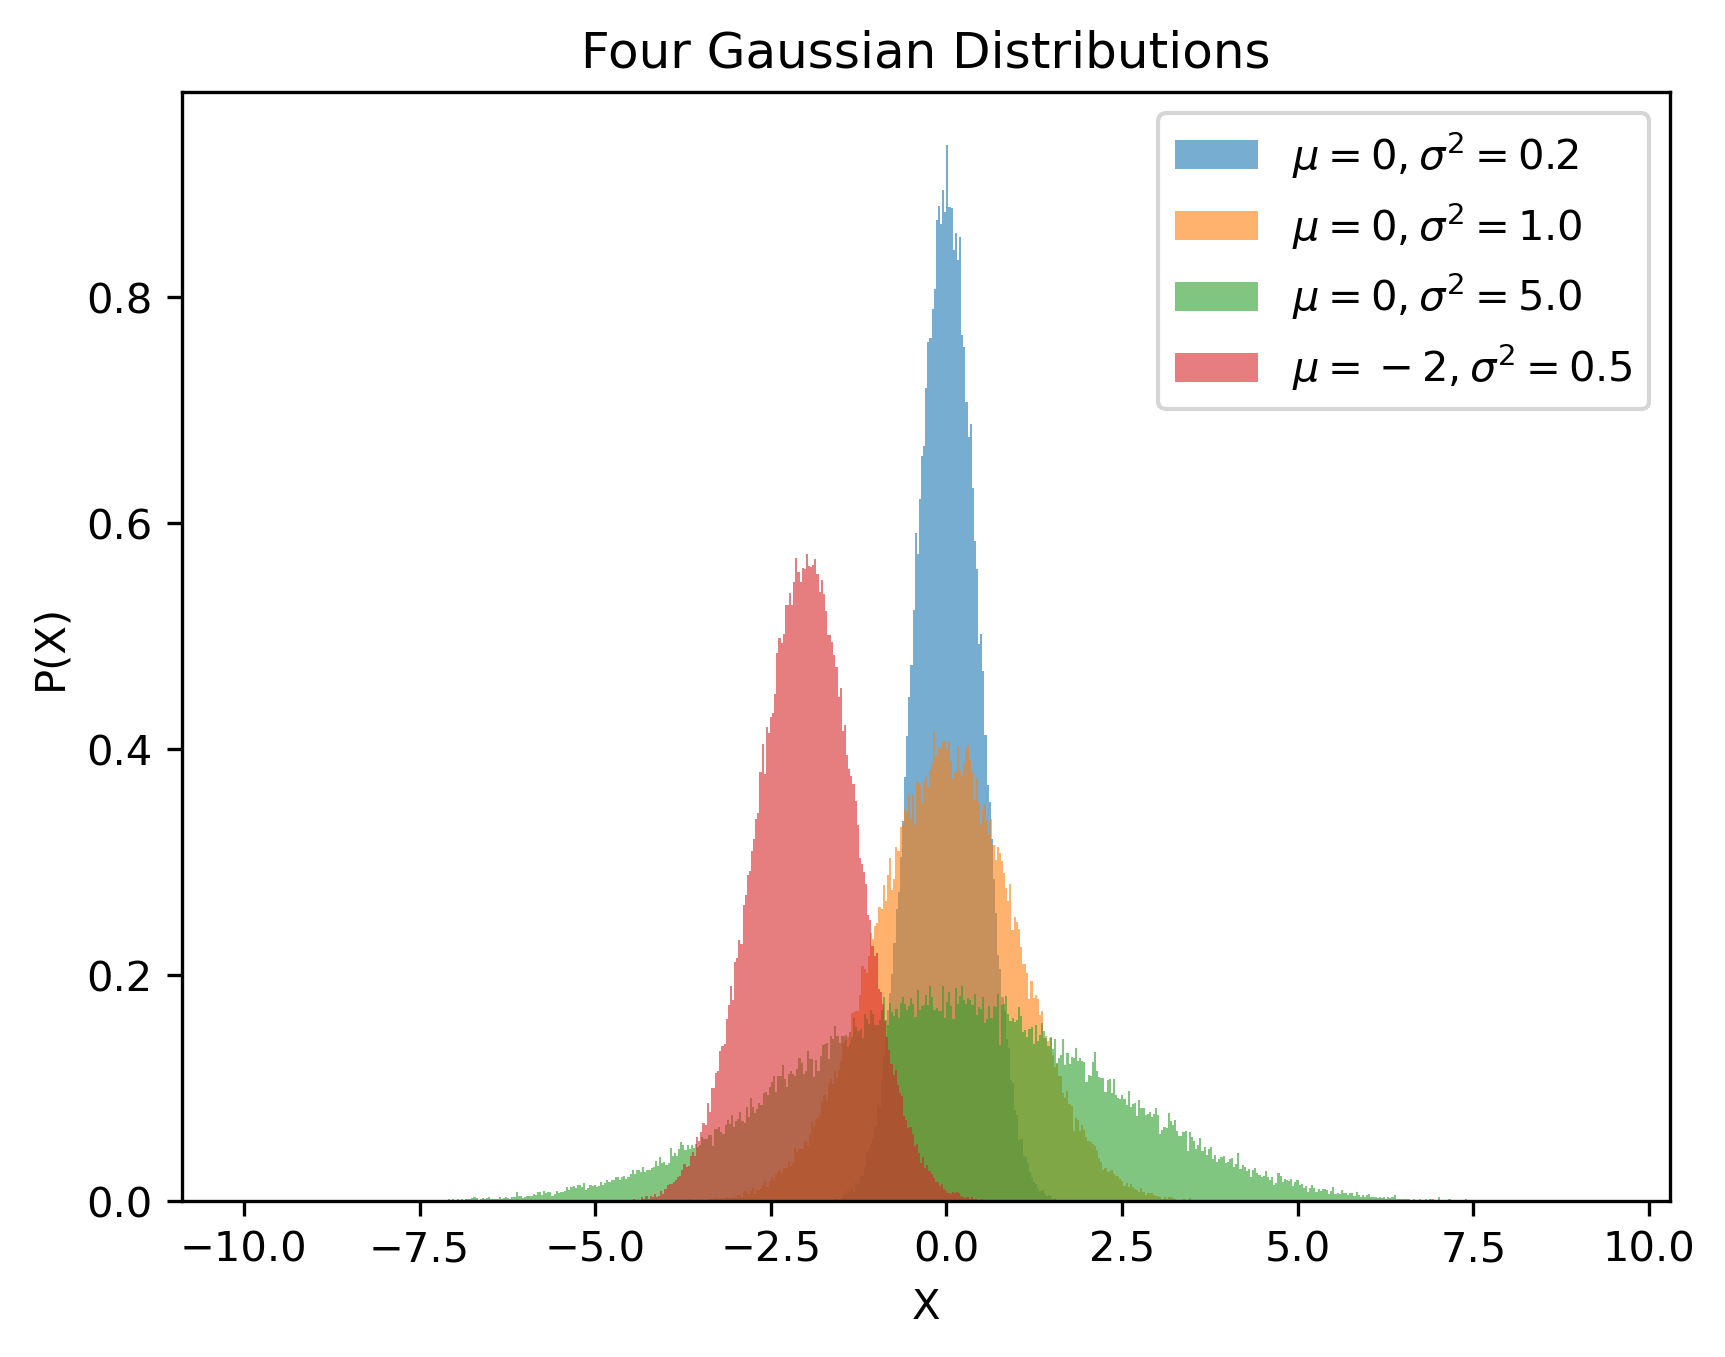
\includegraphics[width=0.6\textwidth]{images/2c.png}
	\caption{Histograms of Gaussian distributions generated using algorithm $\cal{A}$}
\end{figure}

\subsection*{Task D}
\begin{lstlisting}[language=Python, caption={Python code to implement Galton board and plot their histograms for $h=10,50,100$}, label=lst:galton]
import matplotlib as mpl
import matplotlib.pyplot as plt
import numpy as np

mpl.rcParams["figure.dpi"] = 300

N = 10**5
hs = [10, 50, 100]
for i, h in enumerate(hs):
    pockets = []
    for _ in range(N):
        dirs = np.random.randint(2, size=h) # uniformly sample h values from {0, 1}
        x = np.sum(dirs * 2 - 1) # map 0 to -1 and 1 to 1, and sum them to get final pocket
        pockets.append(x)
    plt.hist(pockets, bins=100, density=True)
    plt.xlabel("pocket")
    plt.ylabel("normalized count")
    plt.title(f"Galton board with h={h}")
    plt.savefig(f"2d{i + 1}.png", bbox_inches="tight")
    plt.show()
\end{lstlisting}
\begin{figure}[H]
	\centering
	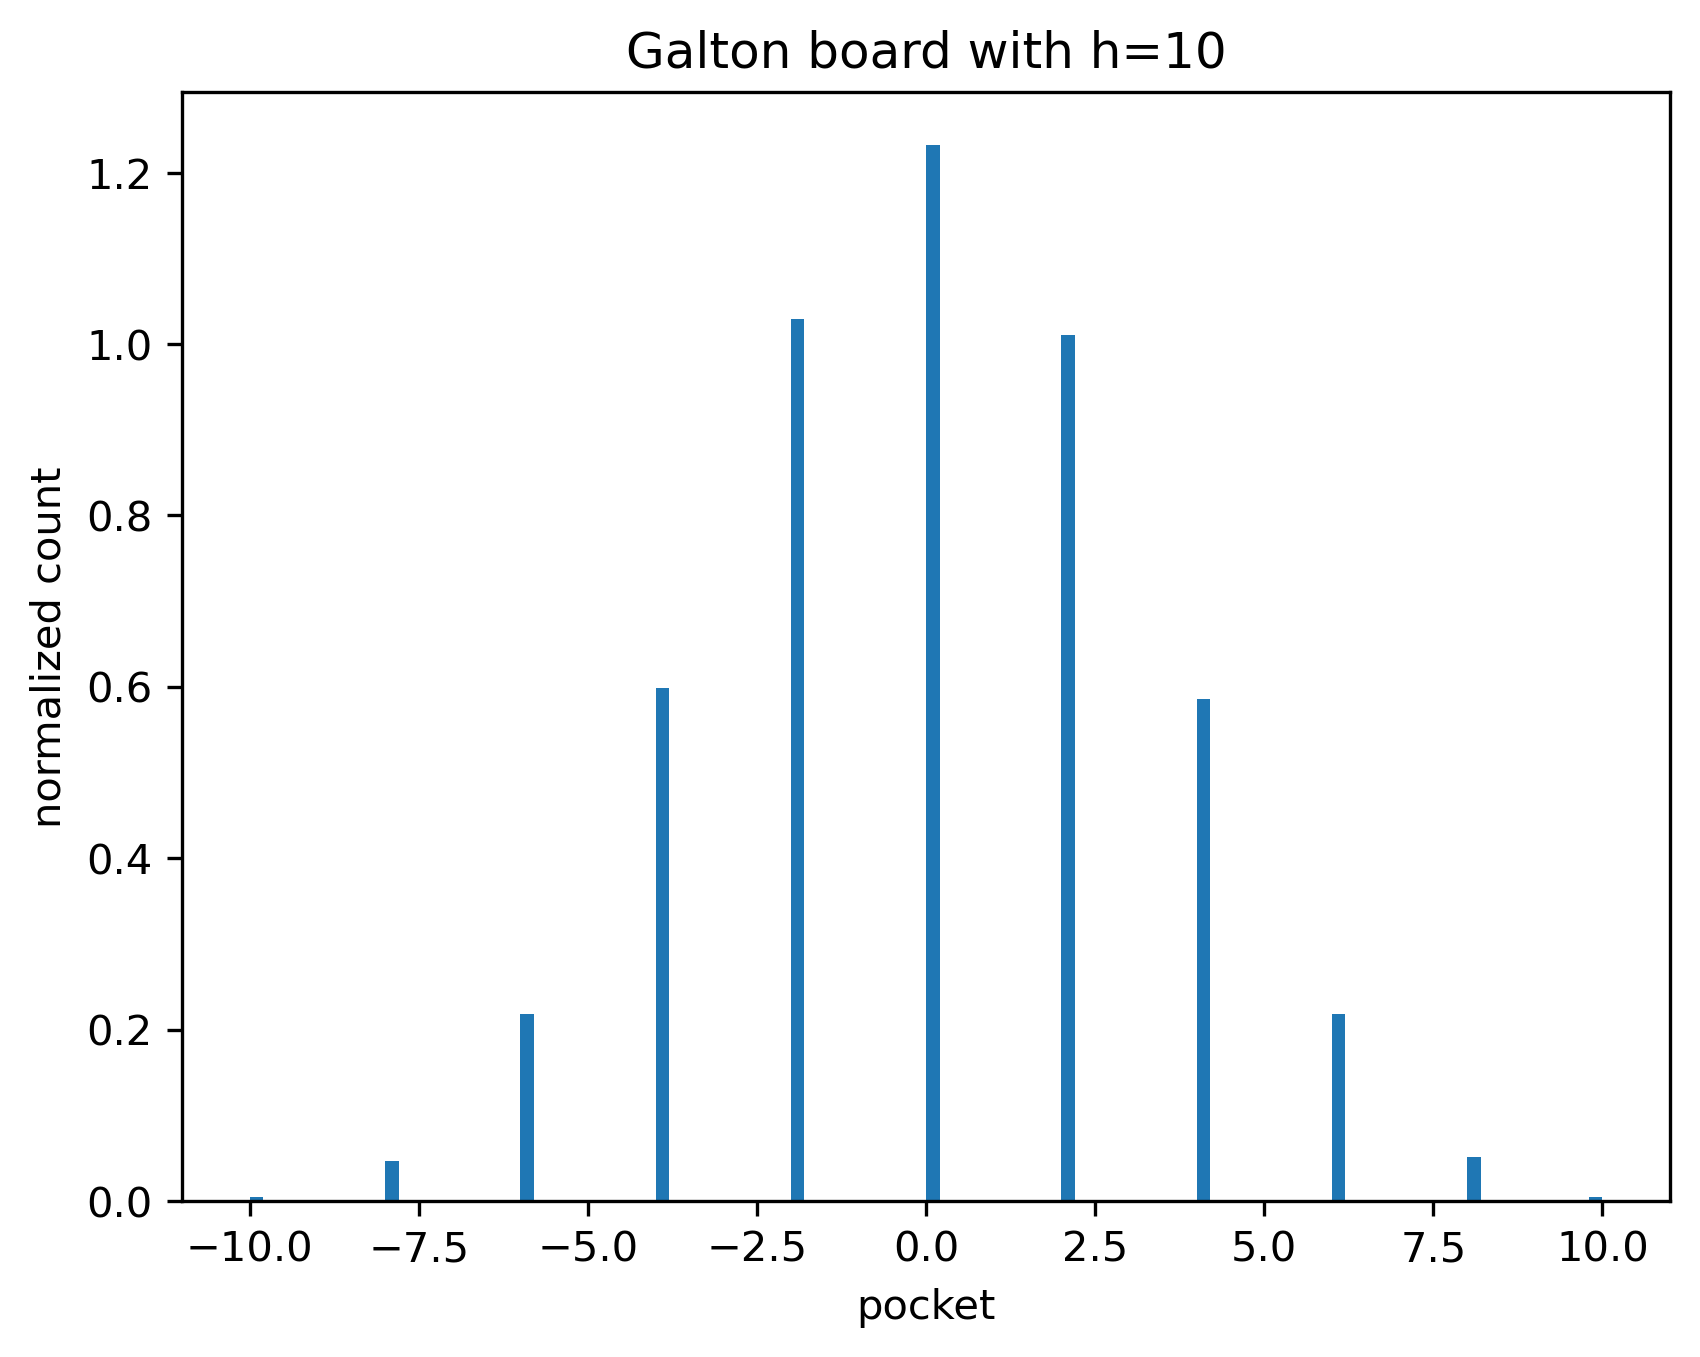
\includegraphics[width=0.6\textwidth]{images/2d1.png}
	\caption{Galton board with $h=10$}
\end{figure}
\begin{figure}[H]
	\centering
	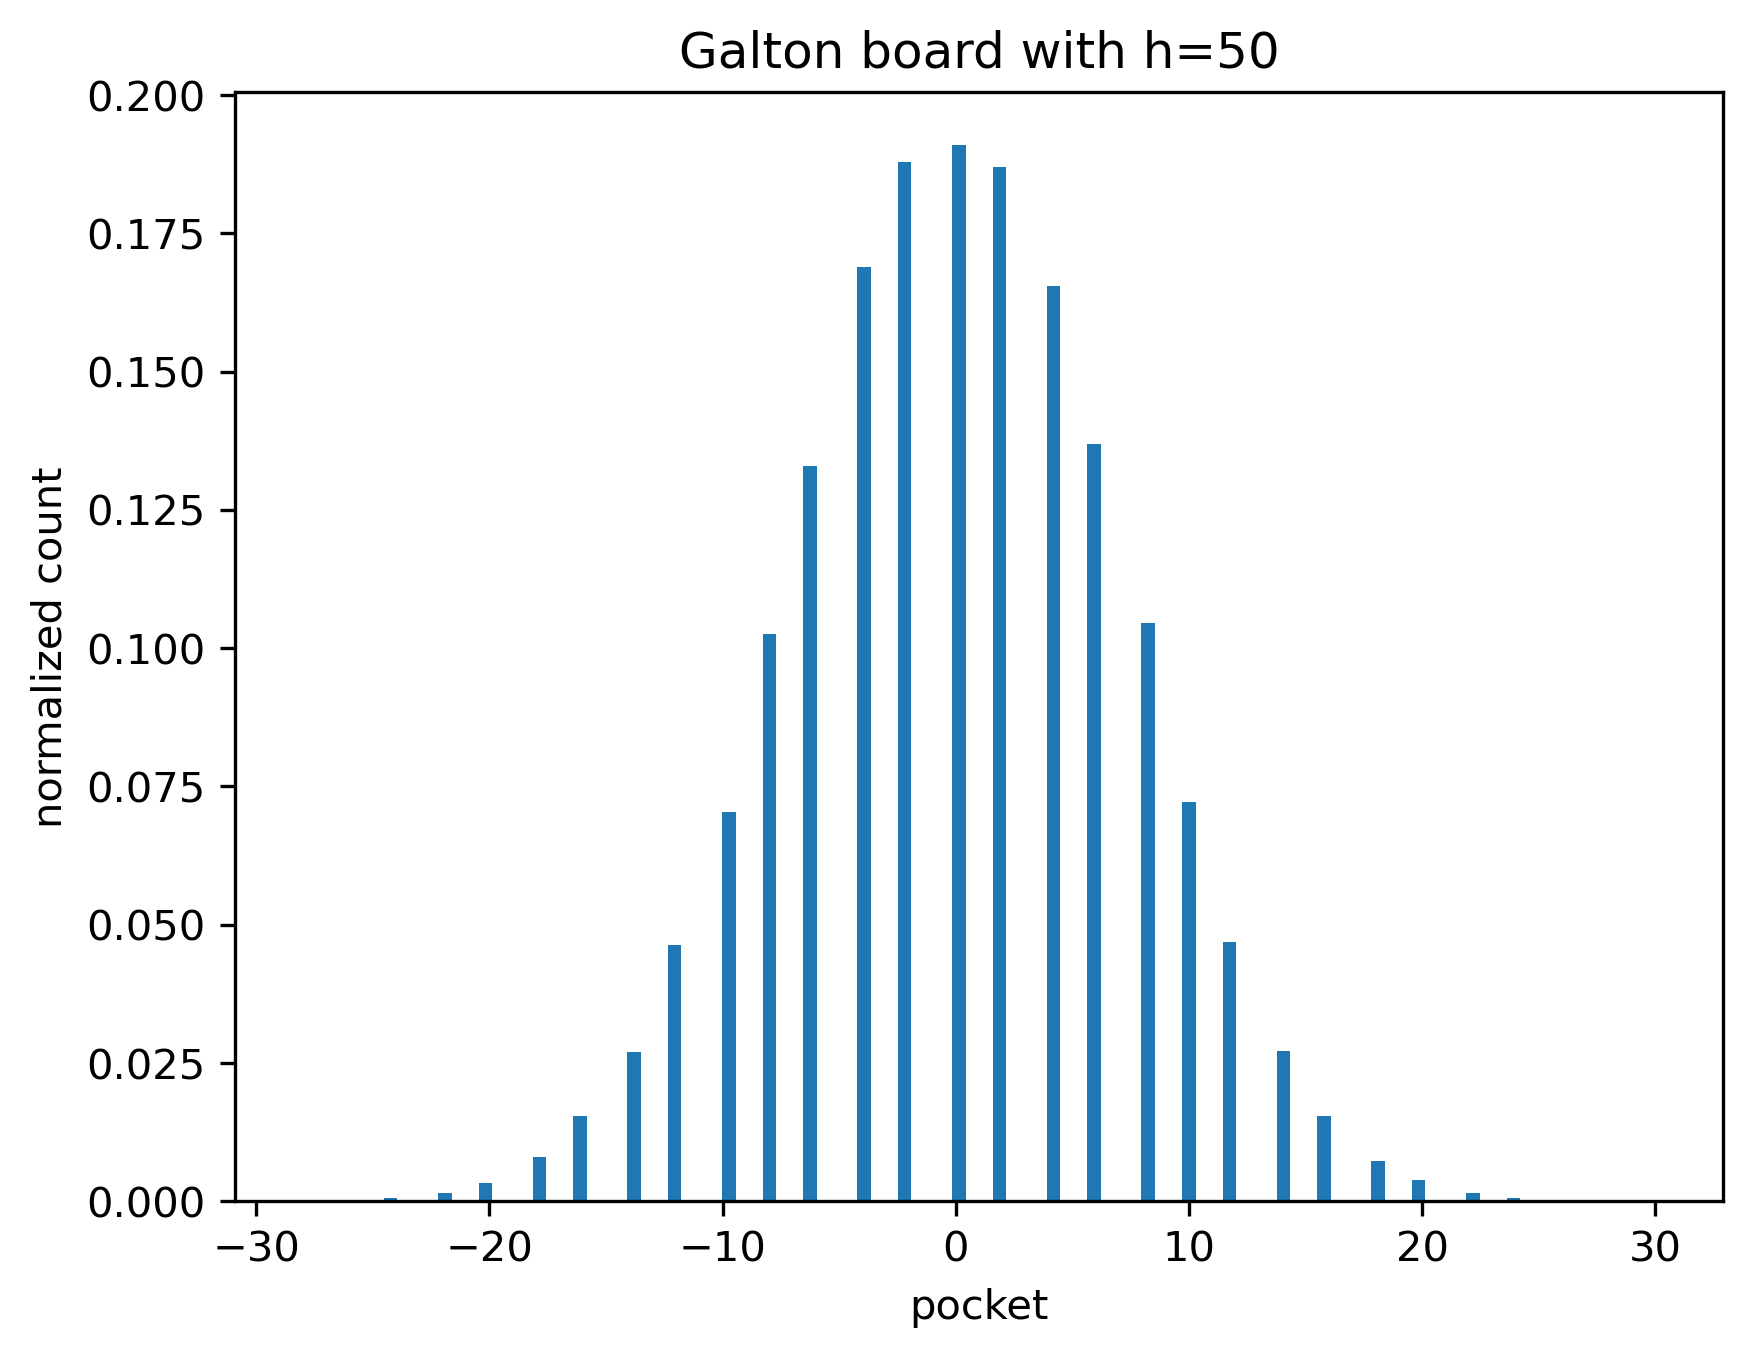
\includegraphics[width=0.6\textwidth]{images/2d2.png}
	\caption{Galton board with $h=50$}
\end{figure}
\begin{figure}[H]
	\centering
	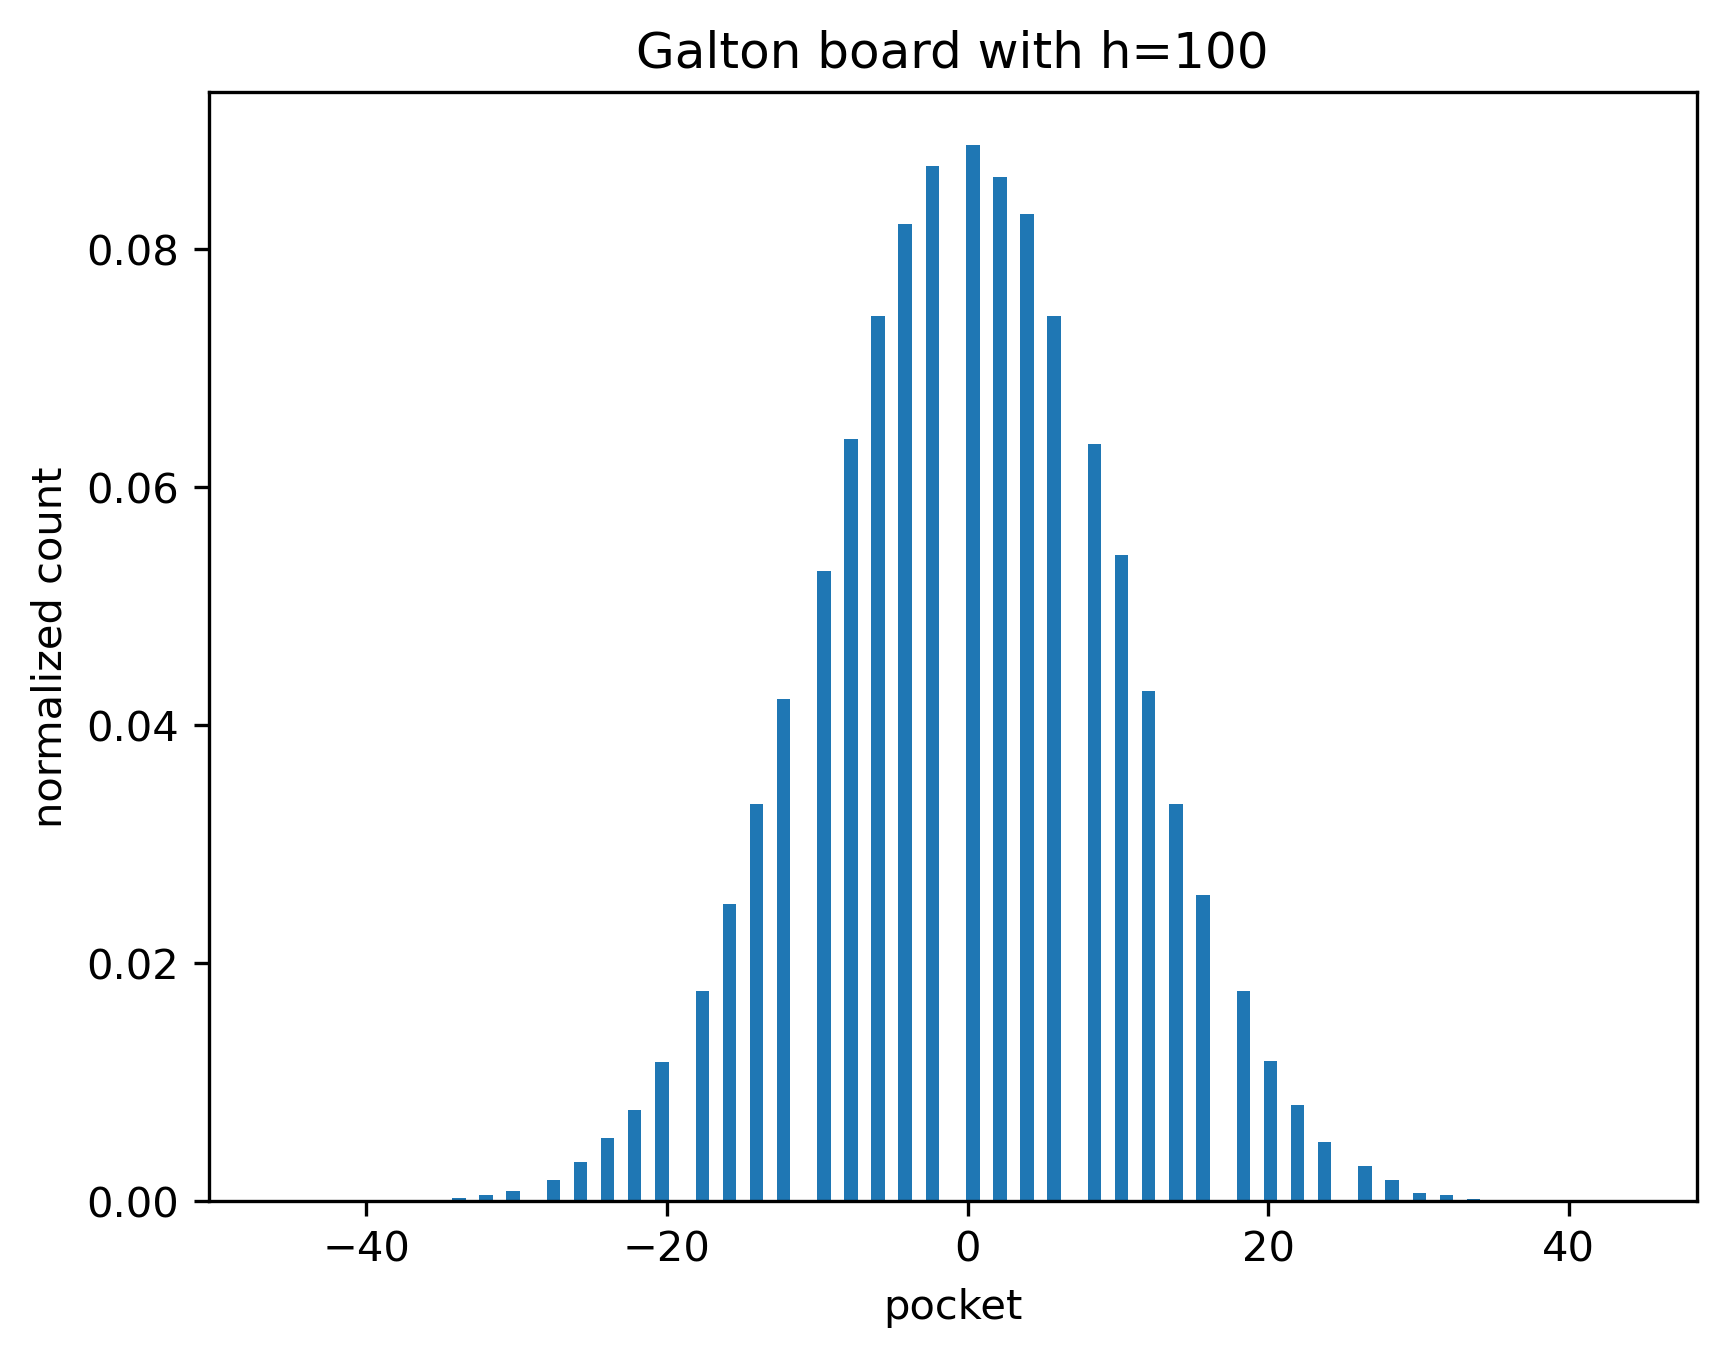
\includegraphics[width=0.6\textwidth]{images/2d3.png}
	\caption{Galton board with $h=100$}
\end{figure}

\subsection*{Task E}
We are given a Galton Board of depth $h$, and random variable $X\in \left\{-h,-h+2,\cdots,0,2,\cdots,h-2,h\right\}$ to describe the pocket in which a ball lands.

\subsubsection*{Computing $P_h[X=2i]$ \normalfont for $i\in\{-k,-k+1,\cdots,k-1,k\}$}
Consider random variable $Y \in \{-1,1\}$, which represents the direction of the ball after hitting a peg, $-1$ for left and $1$ for right.
We have random variables $Y_j$ for $j\in\left\{1,2,\cdots,h\right\}$ representing the directions of the ball after hitting each peg.
Note that $X = \sum_{j=1}^{h}Y_j$.\\

\begin{claim}
	For $X=2i$ and $i \in \left\{-k,-k+1,\cdots, -1,0,1,\cdots,k-1,k\right\}$, we need to have $k - i$ left movements.
\end{claim}
\begin{proof}
	Consider $a$ number of left movements, and $h-a=2k-a$ number of right movements.
	We need to find a solution to the following equation.
	\begin{align*}
		-1 \cdot a + 1 \cdot (2k-a) & = 2i    \\
		2k - 2a                     & = 2i    \\
		\therefore    a             & = k - i
	\end{align*}
	This gives us the number of left movements. Note that $a$ is always non-negative.
\end{proof}

Once we have the number of left movements, we can choose any $k-i$ pegs out of $h$ pegs to be the left movements.
And at each peg, the probability of going left or right is equal to $1/2$.
So, we can write the probability of $X=2i$ as:
\begin{align}
	\therefore P_h[X=2i] = \binom{h}{k-i} \left(\frac{1}{2}\right)^h \label{eq:probx2i}
\end{align}

\subsubsection*{Showing that $P_h$ converges to a Gaussian Distribution}
\begin{remark}
	A couple of well-known approximations that we will use in our proof are:
	\begin{align}
		(1+x)^n & \approx 1 + nx \label{eq:binomial-approx}                                   \\
		e^{-x}  & \approx 1 - x \label{eq:exp-approx}                                         \\
		n!      & \approx \sqrt{2\pi n} \left(\frac{n}{e}\right)^n \label{eq:stirling-approx}
	\end{align}
	\cref{eq:binomial-approx} is valid for $x$ small and $n$ large.
	\cref{eq:exp-approx} is valid for $x$ small.
	\cref{eq:stirling-approx} is valid for large $n$.
\end{remark}
We first substitute $2i$ for $i$, and $k$ for $\dfrac{h}{2}$ in \cref{eq:probx2i}.
\begin{align*}
	P_h[X=i] & = \binom{h}{\frac{h-i}{2}} \left(\frac{1}{2}\right)^h
\end{align*}
Now, we will simplify the binomial coefficient term using \cref{eq:stirling-approx}.
\begin{align*}
	\binom{h}{\frac{h-i}{2}}\left(\frac{1}{2}\right)^h & = \frac{h!}{2^h\left(\frac{h-i}{2}\right)!\left(\frac{h+i}{2}\right)!}                                                                                                                                         \\
	                                                   & \approx \frac{\sqrt{2\pi h}\left(\frac{h}{e}\right)^h}{2^h\sqrt{2\pi \frac{h-i}{2}}\left(\frac{h-i}{2e}\right)^\frac{h-i}{2}\sqrt{2\pi \frac{h+i}{2}}\left(\frac{h+i}{2e}\right)^\frac{h+i}{2}}                \\
	                                                   & = \sqrt{\frac{2\pi h}{\pi(h-i)\pi(h+i)} }\left(\frac{h}{2e}\right)^h \left(\frac{\frac{h-i}{2e}}{\frac{h+i}{2e}}\right)^\frac{i}{2}\left(\frac{1}{\frac{h-i}{2e} \frac{h+i}{2e}}\right)^\frac{h}{2}            \\
	                                                   & = \sqrt{\frac{2 h}{\pi \left(h^2-i^2\right)}}\left(\frac{h}{2e}\right)^h \left(\frac{1-\frac{i}{h}}{1+\frac{i}{h}}\right)^\frac{i}{2}\left(\frac{(2e)^2}{h^2-i^2}\right)^\frac{h}{2}                           \\
	                                                   & = \sqrt{\frac{2 h}{\pi \left(h^2-i^2\right)}}\left(\frac{h}{2e}\right)^h \left(\frac{1-\frac{i}{h}}{1+\frac{i}{h}}\right)^\frac{i}{2}\left(\frac{(2e)^2}{h^2\left(1-\frac{i^2}{h^2}\right)}\right)^\frac{h}{2} \\
	                                                   & = \sqrt{\frac{2 h}{\pi \left(h^2-i^2\right)}}\left(\frac{h}{2e}\right)^h \left(\frac{1-\frac{i}{h}}{1+\frac{i}{h}}\right)^\frac{i}{2}\left(\frac{2e}{h}\right)^h\left(1-\frac{i^2}{h^2}\right)^{-\frac{h}{2}}  \\
	                                                   & = \sqrt{\frac{2 h}{\pi \left(h^2-i^2\right)}} \left(\frac{1-\frac{i}{h}}{1+\frac{i}{h}}\right)^\frac{i}{2}\left(1-\frac{i^2}{h^2}\right)^{-\frac{h}{2}}
\end{align*}
Since we are given that $i << \sqrt{h}$, we can approximate $h^2-i^2 \approx h^2$. Also, we can use \cref{eq:binomial-approx} and \cref{eq:exp-approx} to make the following approximations:
\begin{align*}
	\left(1-\frac{i}{h}\right)^\frac{i}{2}        & \approx 1-\frac{i^2}{2h}  \approx e^{-\frac{i^2}{2h}}  \\
	\left(1+\frac{i}{h}\right)^{-\frac{i}{2}}     & \approx 1 - \frac{i^2}{2h} \approx e^{-\frac{i^2}{2h}} \\
	\left(1-\frac{i^2}{h^2}\right)^{-\frac{h}{2}} & \approx 1 + \frac{i^2}{2h} \approx e^\frac{i^2}{2h}
\end{align*}
Now, we simply the expression with the new approximations.
\begin{align*}
	\binom{h}{\frac{h-i}{2}}\left(\frac{1}{2}\right)^h & \approx \sqrt{\frac{2 h}{\pi h^2}}e^{-\frac{i^2}{2h}}e^{-\frac{i^2}{2h}}e^{\frac{i^2}{2h}} \\
	                                                   & = \sqrt{\frac{2}{\pi h}} e^{-\frac{i^2}{2h}}                                               \\
	\therefore P_h[X=i]                                & \approx \frac{1}{\sqrt{\pi k}} e^{-\frac{i^2}{4k}}
\end{align*}
This shows that the distribution of $X$ converges to a Gaussian distribution as $h$ increases.


% jisne complete nahi kiya vo bhen ka loda
\section{Higher-Order Regression}

\subsection{1}
\begin{claim}
    In a simple linear regression model the point \((\overline{x},\overline{y})\) lies exactly on the least squares regression line.
\end{claim}
\begin{proof}
In a simple linear regression model, the least squares regression line is given by the equation:
\begin{align*}
    y &= Bx + A
\end{align*}
where \(B\) and \(A\) are calculated as:
\begin{align}
    B&=\frac{\sum(x_i-\overline{x})(y_i-\overline{y})}{\sum(x_i - \overline{x})^2}\\
    A&= \overline{y} - B\overline{x}\\
    \therefore y &= Bx + ( \overline{y} - B\overline{x} )
\end{align}

It is now trivial to see that point \((\overline{x},\overline{y})\) lies perfectly on the least square regression line.
\end{proof}

\subsection{2}
\begin{claim}
    The least square estimates of \(\beta_0^* = \overline{y}\) and \(\beta_1^* = \beta_1\)
\end{claim}
\begin{proof}
    In a simple linear regression model:
    \begin{align*}
        Y &= \beta_0 + \beta_1x + \epsilon\\
        \beta_1 &= \frac{\sum(x_i - \overline{x})(y_i-\overline{y})}{\sum(x_i - \overline{x})^2}\\
        \beta_0 &= \overline{y} - \beta_1\overline{x}
    \end{align*}
    while in the new model using \(z_i = x_i - \overline{x}\)
    \begin{align*}
        Y &= \beta_0^* + \beta_1^*z + \epsilon
    \end{align*}
    Using the formulae for a simple linear regression model the least square estimates of \(\beta_0^*\) and \(\beta_1^*\) are:
    \begin{align*}
        \beta_1^* &= \frac{\sum(z_i-\overline{z})(y_i-\overline{y})}{\sum(z_i - \overline{z})^2}\\
        \beta_1^* &= \frac{\sum(z_i)(y_i-\overline{y})}{\sum(z_i)^2}\\
        \beta_1^* &= \frac{\sum(x_i - \overline{x})(y_i-\overline{y})}{\sum(x_i - \overline{x})^2}\\
        \beta_1^* &= \beta_1\\
        \beta_0^* &= \overline{y} - \beta_1^*\overline{z}\\
        \beta_0^* &= \overline{y} - \beta_1^*(0)\\
        \beta_0^* &= \overline{y}
    \end{align*}
    In summary, the models are mathematically equivalent in terms of fitting the data, but the interpretation of the intercept changes. The transformed model centers the data, making the intercept equal to the mean of Y, while the slope remains the same in both models
\end{proof}

\subsection{3}
The data was run through OLS with validation split 90:10\\
\vspace{-2em}
\begin{figure}[H]
    \centering
    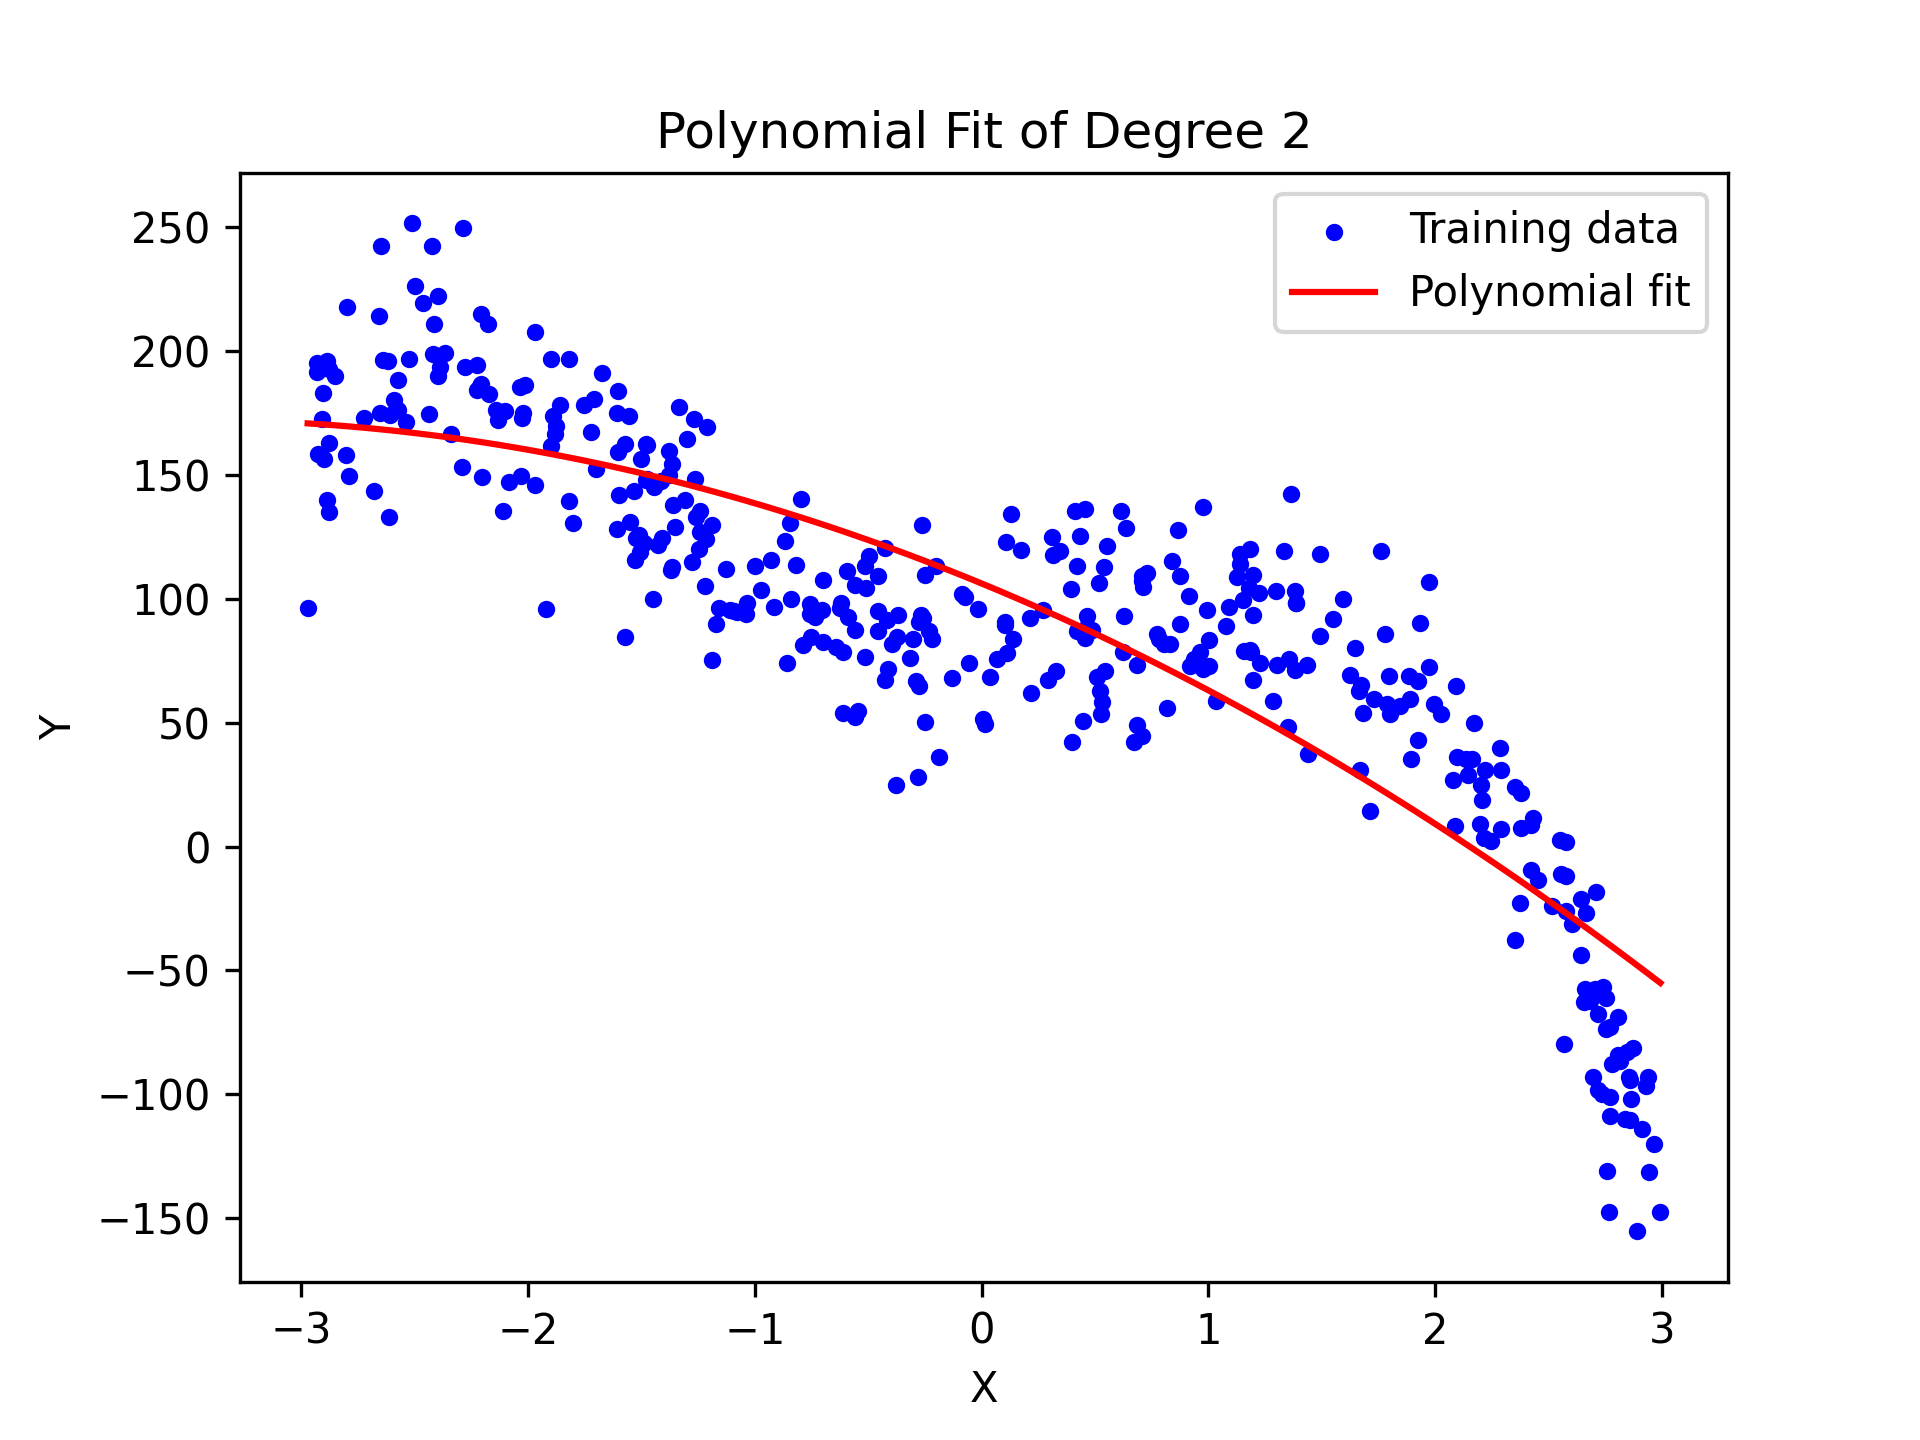
\includegraphics[width=0.5\textwidth]{./images/3/3_underfit.png}
    \vspace{-10pt}
    \caption{Underfit}
\end{figure}
\vspace{-15pt}
\begin{figure}[H]
    \centering
    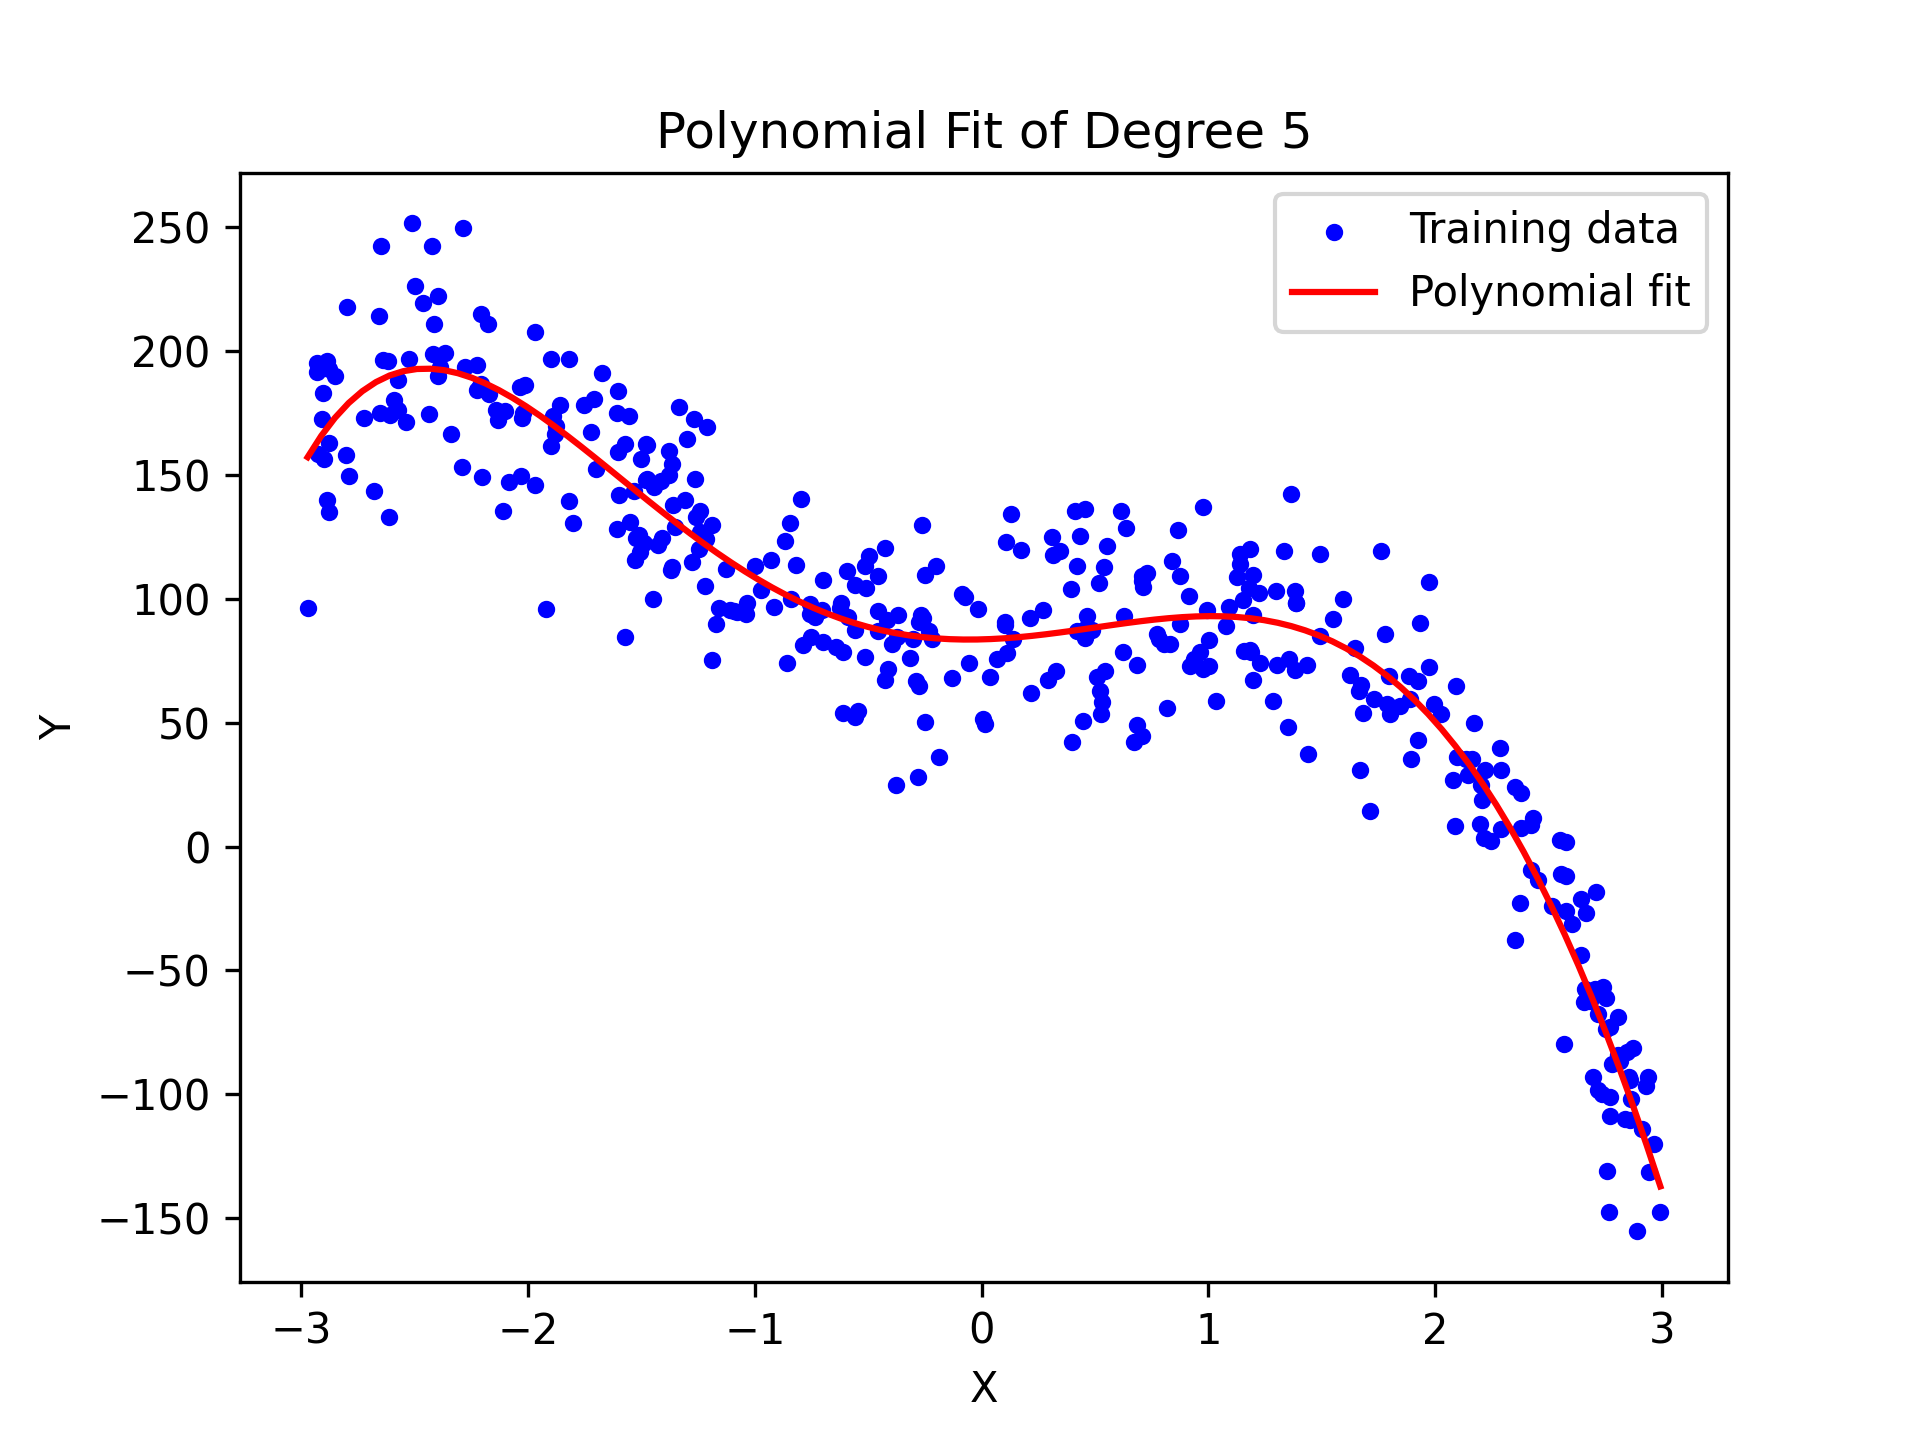
\includegraphics[width=0.5\textwidth]{./images/3/3_correctfit.png}
    \vspace{-10pt}
    \caption{Correct Fit}
\end{figure}
\vspace{-15pt}
\begin{figure}[H]
    \centering
    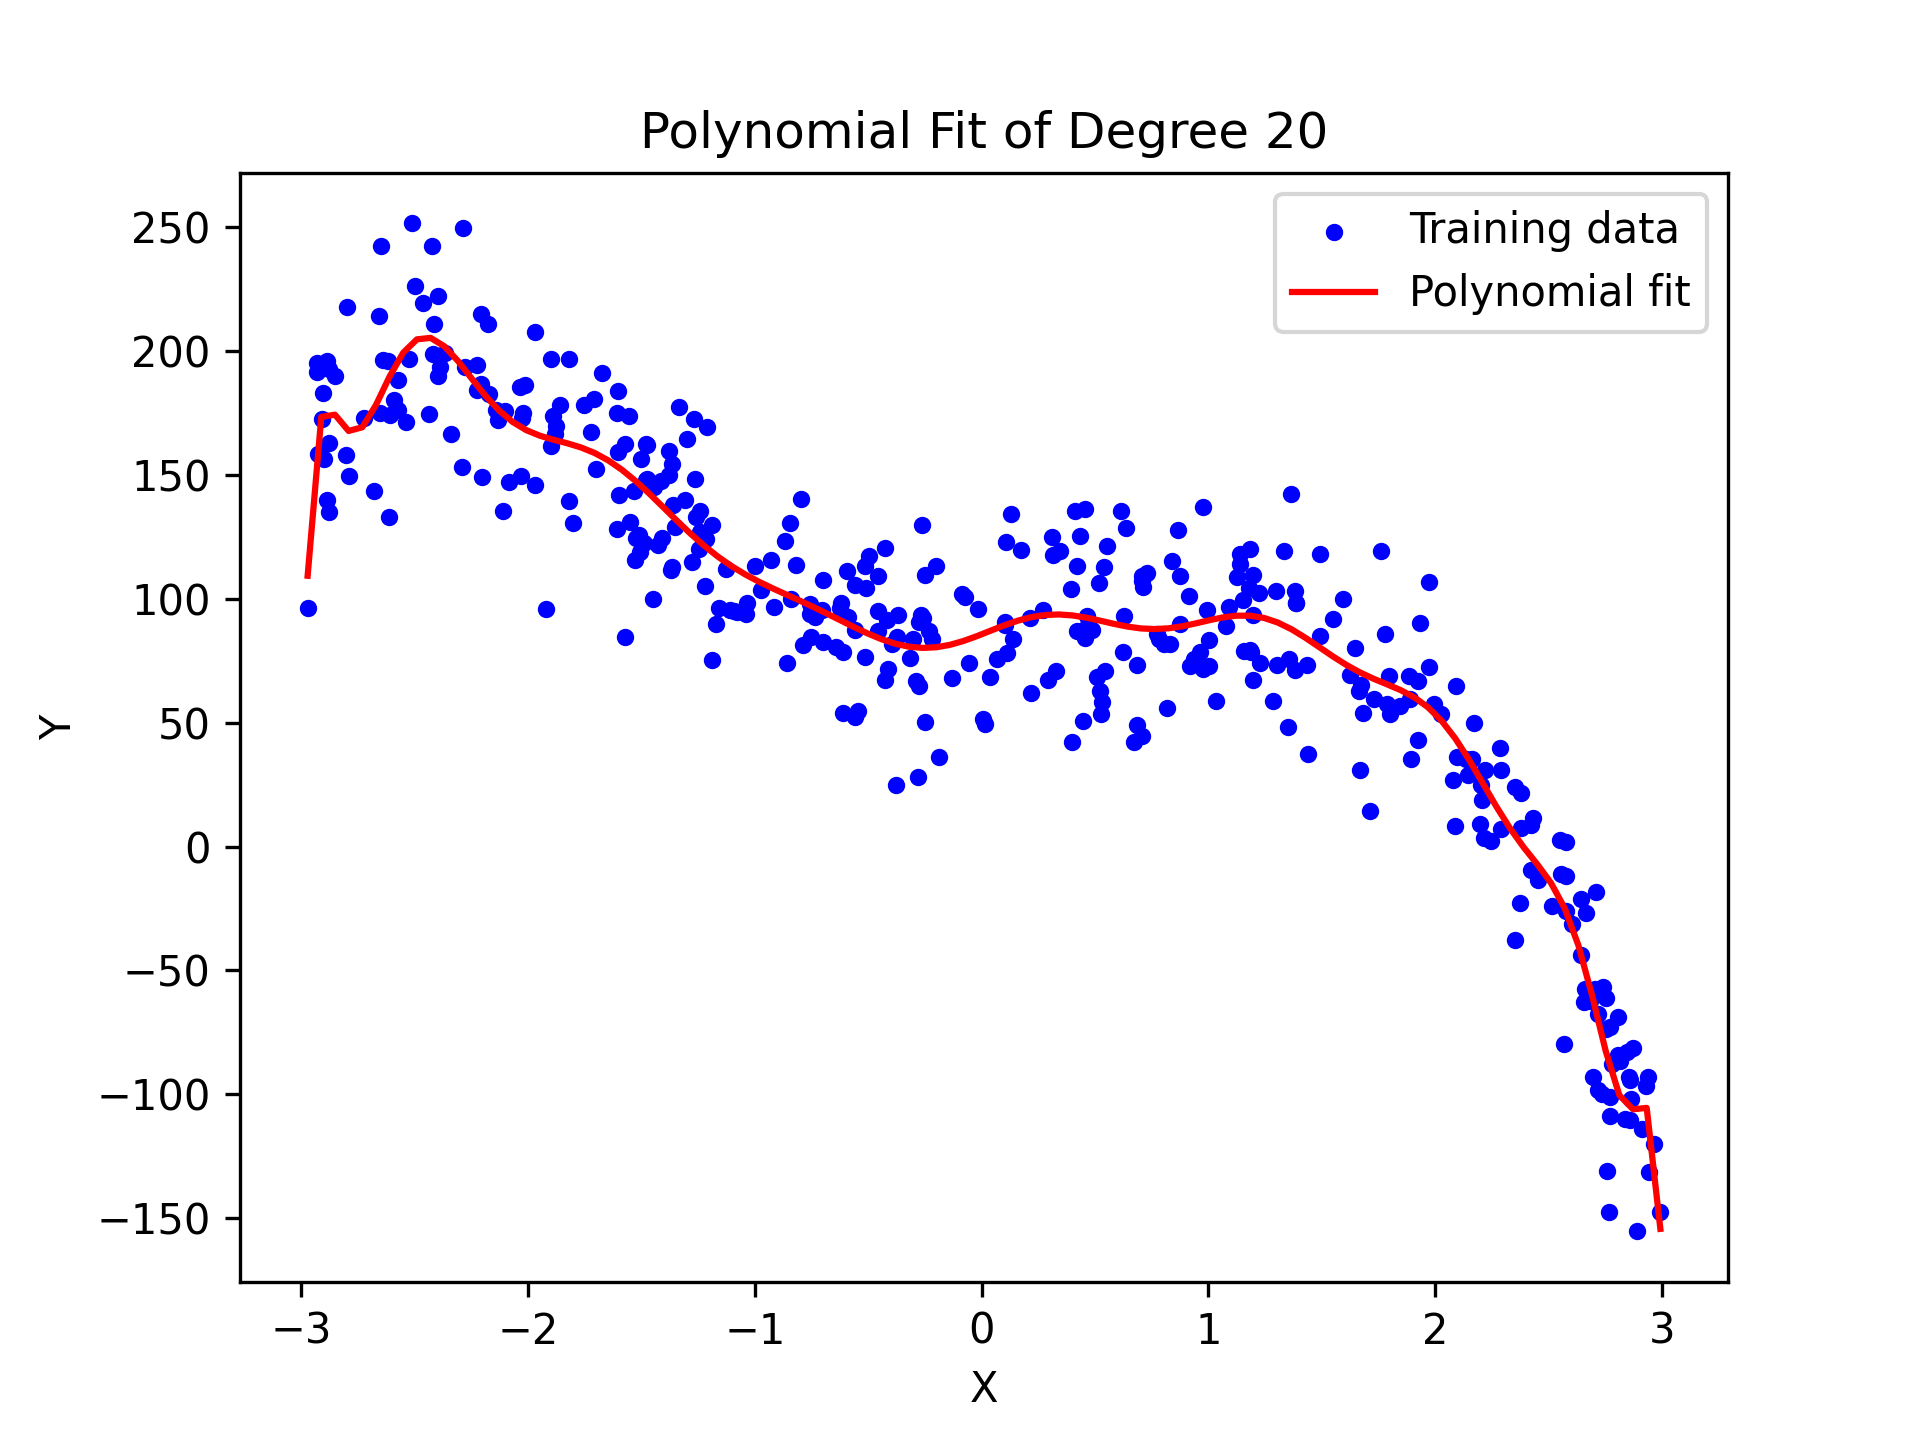
\includegraphics[width=0.5\textwidth]{./images/3/3_overfit.png}
     \vspace{-10pt}
    \caption{Overfit}
\end{figure}


\begin{center}    
    \begin{tabular}{|c|c|c|}
        \hline
        \bf{Degree Of Polynomial} & \bf{Type of Fit} & \bf{Coefficient Of Determination}\\
        \hline
        2 & Underfit & 0.8764 \\
        5 & Correct Fit & 0.9517\\
        20 & Overfit & 0.9545\\
        \hline
    \end{tabular} 
\end{center}
\section{Quality in Inequalitites}

\section{Multivariate Insights Unlocked!}
\section{Update Functions}
All following results assume $1$-based indexing. However, the code written below follows $0$-based indexing.
\begin{itemize}
	\item Old mean:
	      \[
		      \mu = \frac{\sum_{i = 1}^{n} x_i}{n}
	      \]
	      Updated mean:
	      \[
		      \mu' = \frac{\sum_{i = 1}^{n + 1} x_i}{n + 1}
	      \]
	      We can split the term $\sum_{i = 1}^{n + 1} = \sum_{i = 1}^{n} + x_{n + 1} = n\mu + x_{n+1}$
	      \[
		      \mu' = \frac{n\mu + x_{n+1}}{n+1}
	      \]
	\item Old median:
	      \[
		      \text{In sorted Array A of even length, median = } (A[n/2 + 1] + A[n/2]) / 2
	      \]
	      \[
		      \text{In sorted Array A of odd length, median = } A[(n+1)/2]
	      \]
	      Updated median:
	      \[
		      \text{In a sorted array of even length, median } =
		      \begin{cases}
			      \text{\texttt{NewData}} & \text{if \texttt{NewData} lies between } A[n/2] \text{ and } A[n/2 + 1] \\
			      A[n/2]                  & \text{if \texttt{NewData} is less than } A[n/2]                         \\
			      A[n/2 + 1]              & \text{if \texttt{NewData} is greater than } A[n/2 + 1]
		      \end{cases}
	      \]

	      \[
		      \text{In a sorted array of odd length, median } =
		      \begin{cases}
			      \frac{A[(n+1)/2] + A[(n-1)/2]}{2}              & \text{if \texttt{NewData} } \leq A[(n-1)/2]                        \\
			      \frac{A[(n+1)/2] + A[(n+3)/2]}{2}              & \text{if \texttt{NewData} } \geq A[(n+3)/2]                        \\
			      \frac{A[(n+1)/2] + \text{\texttt{NewData}}}{2} & \text{if } A[(n-1)/2] \leq \text{\texttt{NewData}} \leq A[(n+3)/2]
		      \end{cases}
	      \]
	\item Old Standard Deviation:
	      \[
		      \sigma^2 = \frac{(\sum_{i = 1}^{n} x_i^2) - n\mu^2}{n - 1}
	      \]
	      New Standard Deviation:
	      \[
		      \sigma'^2 = \frac{(\sum_{i = 1}^{n+1} x_i^2) - (n+1)\mu'^2}{n}
	      \]
	      We can split the term $\sum_{i = 1}^{n + 1}x_i^2 = \sum_{i = 1}^{n}x_i^2 + x_n^2$
	      \[
		      \sigma'^2 = \frac{(n - 1)\sigma^2 + n\mu^2 + x_n^2 - (n + 1)\mu'^2}{n}
	      \]
	      \begin{lstlisting}[language=Python, caption={Python code to calculate new Mean, Median and Standard deviation}]
def newMean (OldMean: float, NewDataValue: float, n: int, A: list[float]) -> float:
    oldSum = OldMean * n
    newSum = oldSum + NewDataValue
    return newSum / (n + 1)

def newMedian (OldMedian: float, NewDataValue: float, n: int, A: list[float]) -> float:
    # Assuming sorted list A
    if n % 2 == 0:
        if A[n // 2 - 1] <= NewDataValue <= A[n // 2]:
            return NewDataValue
        elif NewDataValue < A[n // 2 - 1]:
            return A[n // 2 - 1]
        else:
            return A[n // 2]
    else:
        if NewDataValue <= A[n // 2 - 1]:
            return (A[n // 2 - 1] + A[n // 2]) / 2
        elif NewDataValue >= A[n//2 + 1]:
            return (A[n // 2] + A[n // 2 + 1]) / 2
        else:
            return (A[n // 2] + NewDataValue) / 2

def newStd (OldMean: float, OldStd: float, NewMean: float, NewDataValue: float, n: int, A: list[float]) -> float:
    oldSquareSum = ((OldStd ** 2) * (n - 1)) + (n * (OldMean ** 2))
    newSquareSum = oldSquareSum + (NewDataValue ** 2)
    return ((newSquareSum - ((n + 1) * (NewMean) ** 2)) / n) ** 0.5
    \end{lstlisting}
	      To update the histogram, we check which bin \texttt{NewData} lies in. If no such bin exists, we create a new one with just \texttt{NewData}.
\end{itemize}

\section{Plots}
\begin{itemize}
	\item \textbf{Violin Plot:} These plots represent the density of data as the width at that section. The mean and median of the dataset can be seen clearly. It also shows the symmetry/skewness of the dataset based on the wideness on either side. It shows if the dataset has multiple peaks. It also allows us to compare groups by showing them side by side. It can be used for pharmaceutical trials, ecological studies, financial analysis and quality control.
	      \begin{figure}[H]
		      \centering
		      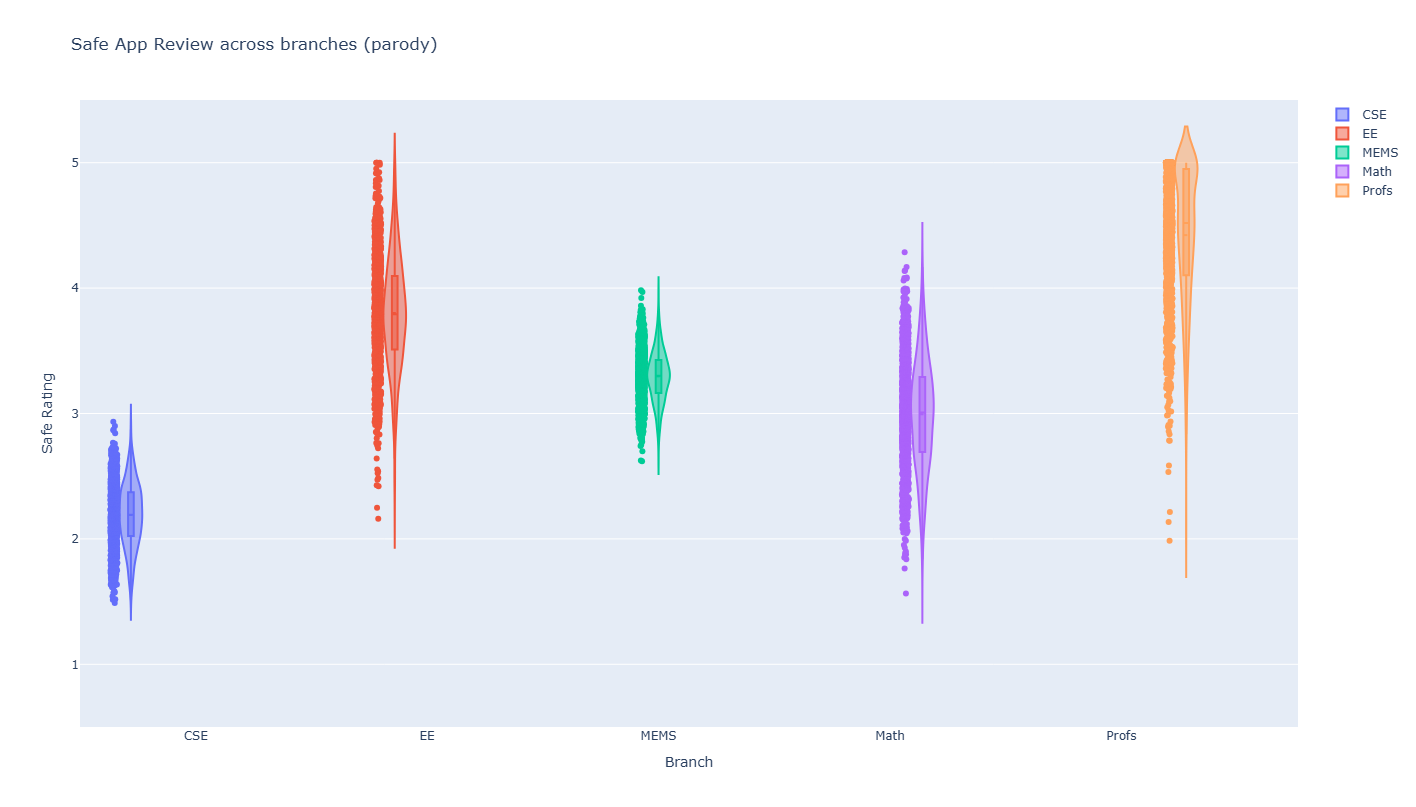
\includegraphics[width=0.85\linewidth]{img/violin.png}
		      \caption{Violin Plot}
	      \end{figure}
	\item \textbf{Pareto Plot:} A Pareto chart is a type of bar chart where each category is represented by a vertical bar. The bars are arranged in descending order of frequency or magnitude from left to right. A cumulative line is often superimposed on the chart to show the total impact of all categories combined. Pareto charts are used to identify the most significant factors in a dataset, typically following the 80/20 rule, where 80\% of the effects come from 20\% of the causes. They are commonly used in quality control, project management, and process improvement to prioritize issues or root causes.
	      \begin{figure}[H]
		      \centering
		      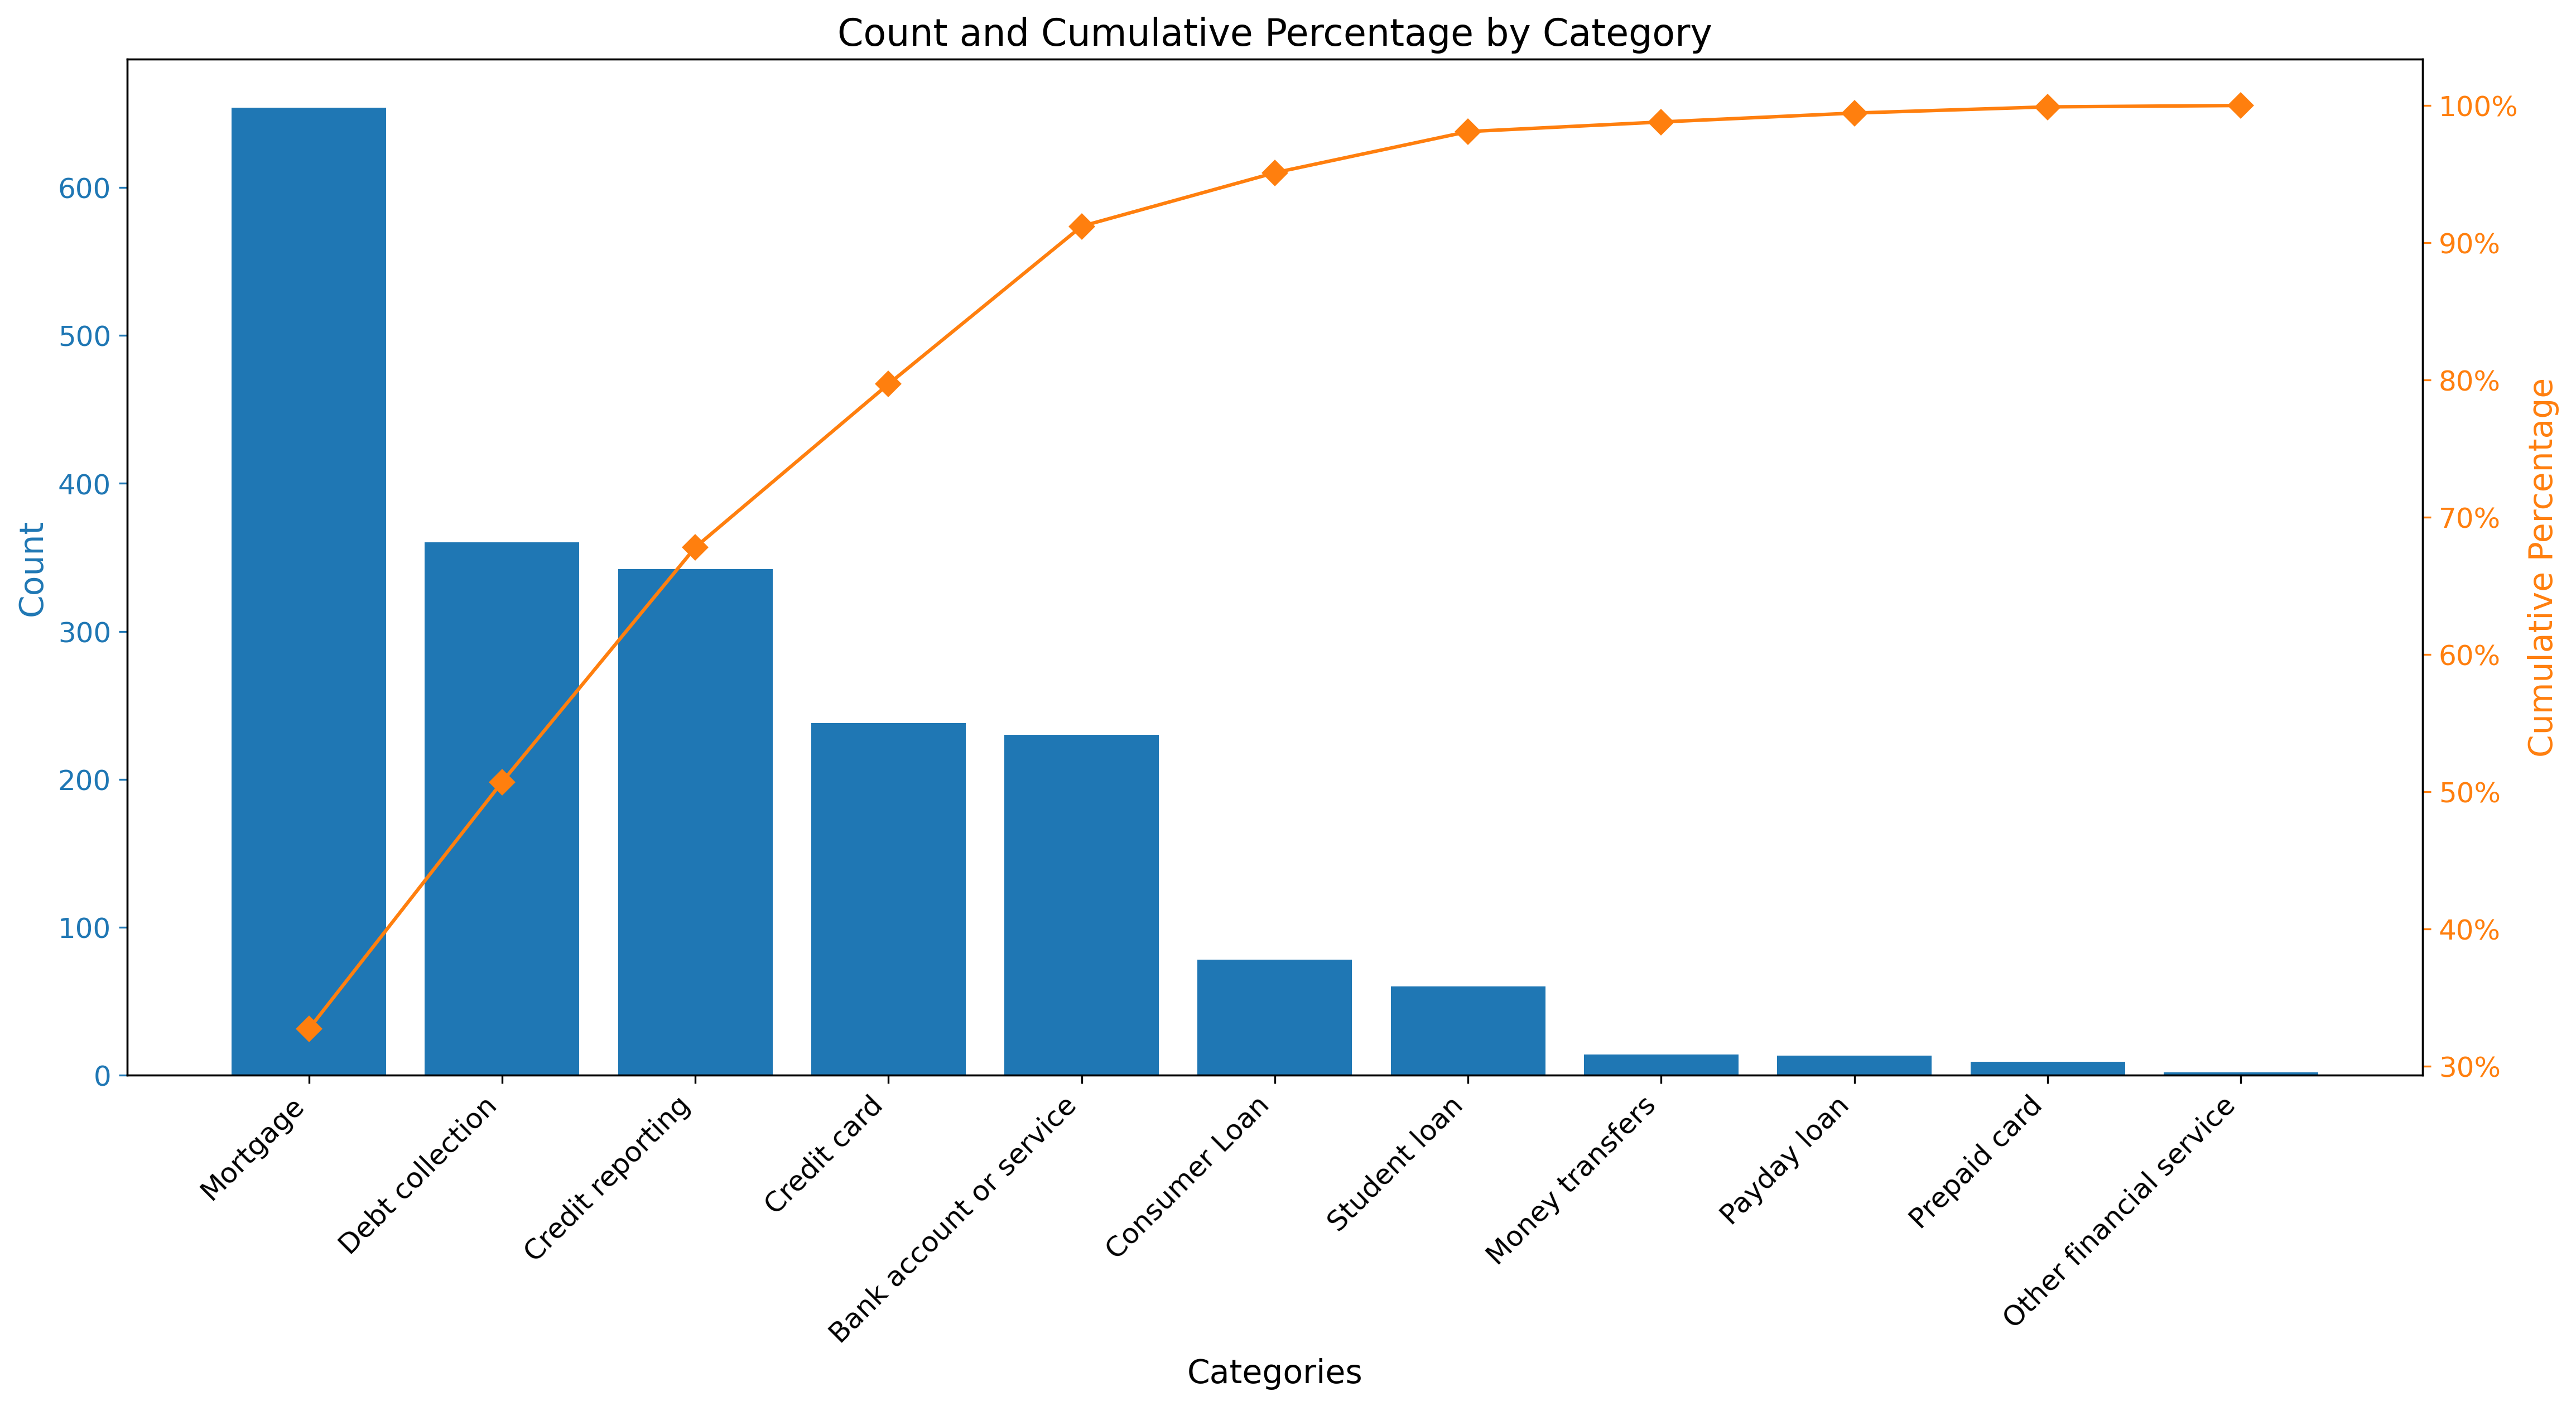
\includegraphics[width=0.85\linewidth]{img/pareto.png}
		      \caption{Pareto Plot, data from \cite{SelenerConsumerComplaints}}
	      \end{figure}
	\item \textbf{Waterfall Plot:} A waterfall plot is a three-dimensional visualization technique commonly used to display changes in signal intensity, frequency, or other continuous variables over time. Each point on the plot represents data at a given time, with the x-axis typically showing time or another independent variable, the y-axis displaying the frequency or another dependent variable, and color or intensity representing the magnitude of the data. Waterfall plots are frequently used in fields such as signal processing, spectroscopy, and audio analysis to monitor how data evolves over time, offering a clear view of trends, patterns, and fluctuations.
	      \begin{figure}[H]
		      \centering
		      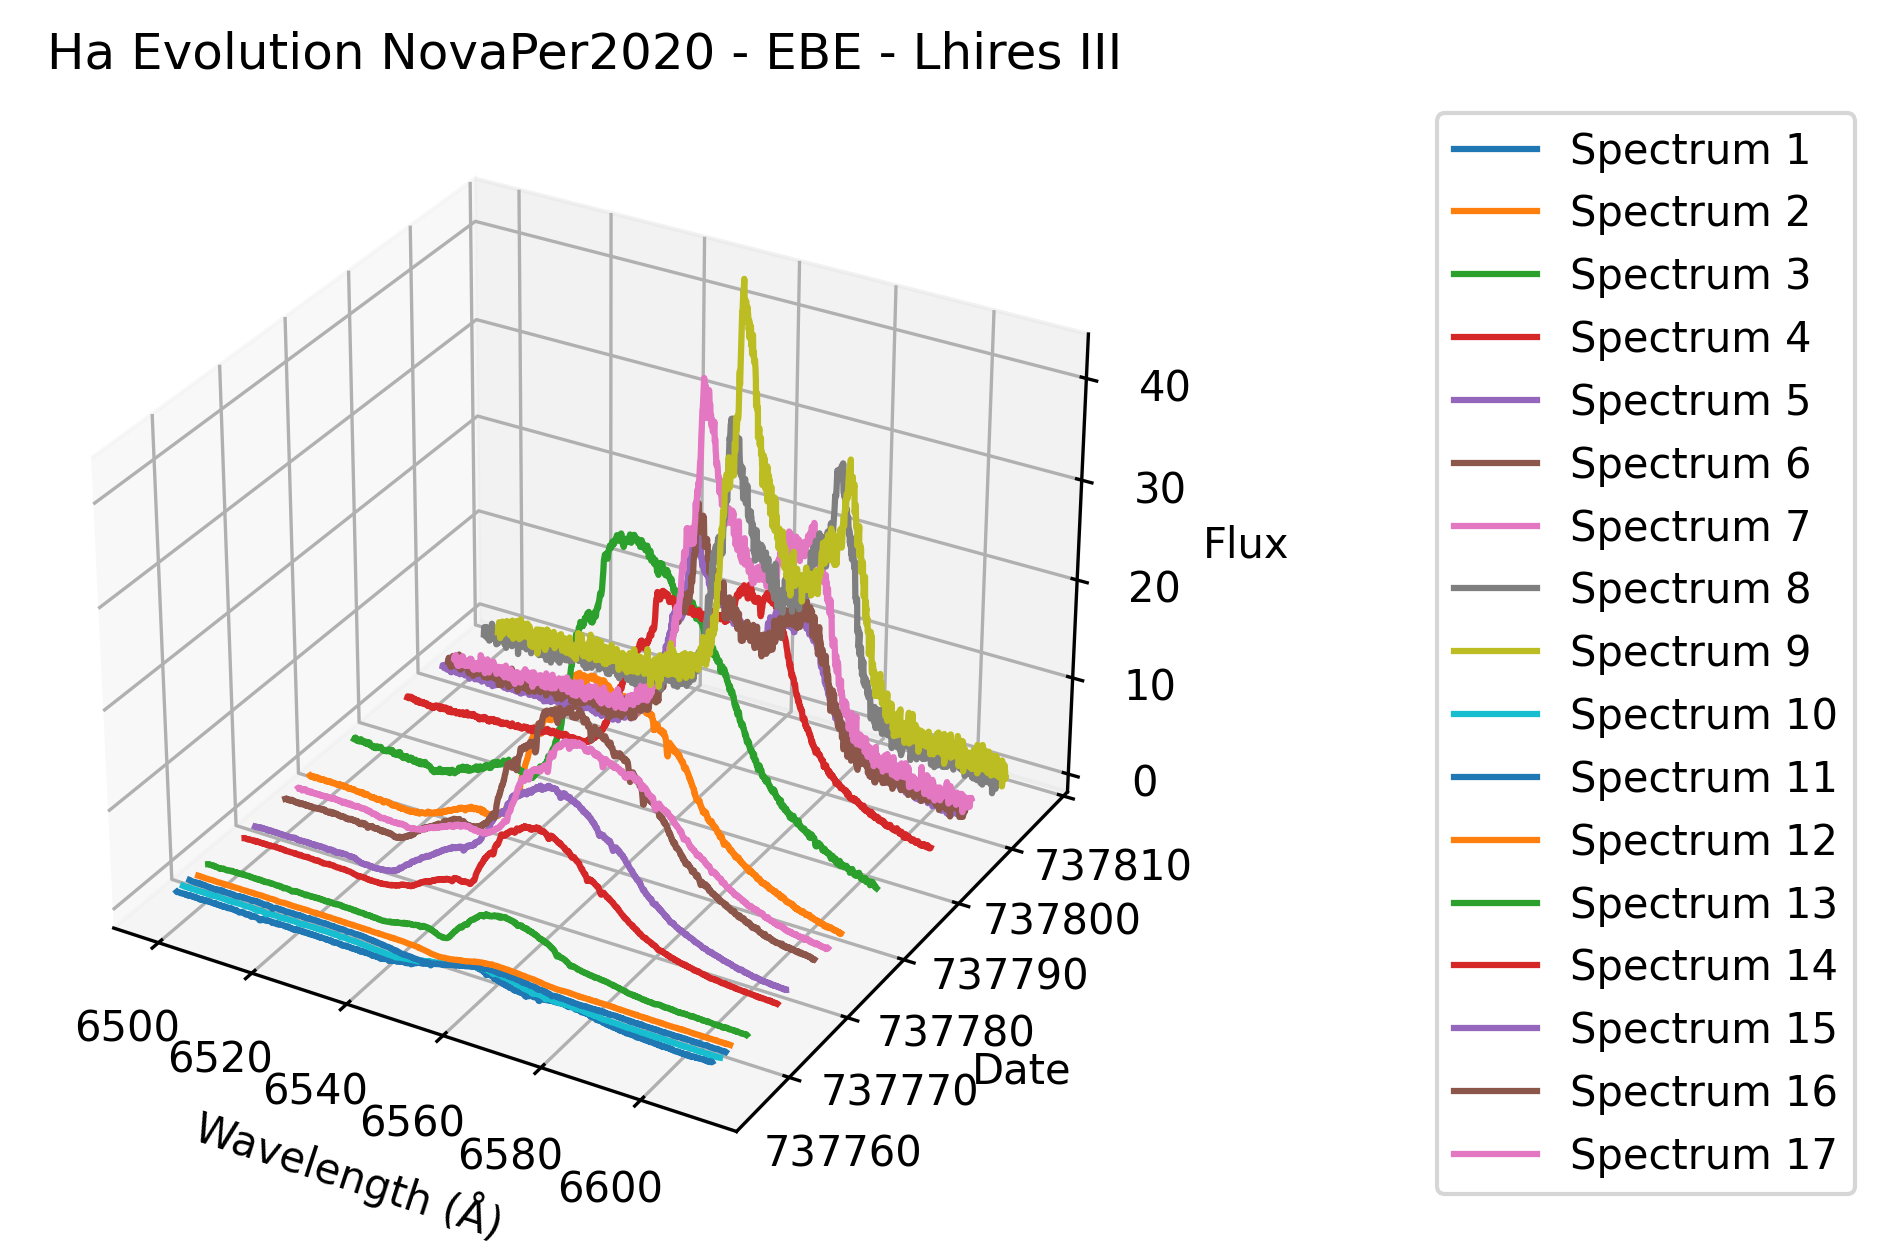
\includegraphics[width=0.8\linewidth]{img/waterfall.png}
		      \caption{Waterfall Plot, data from \cite{Spec3DData}}
	      \end{figure}
	\item \textbf{Coxcomb Plot:} These plots represent data in a circular layout where each category is represented by a wedge. All wedges have the same angular width. Larger areas and longer radii represent larger values and colours are used to represent different time periods. They are used to represent data that changes cyclically like financial performance over the quarters, monthly rainfall or performance of sports players over a season.
	      \begin{figure}[H]
		      \centering
		      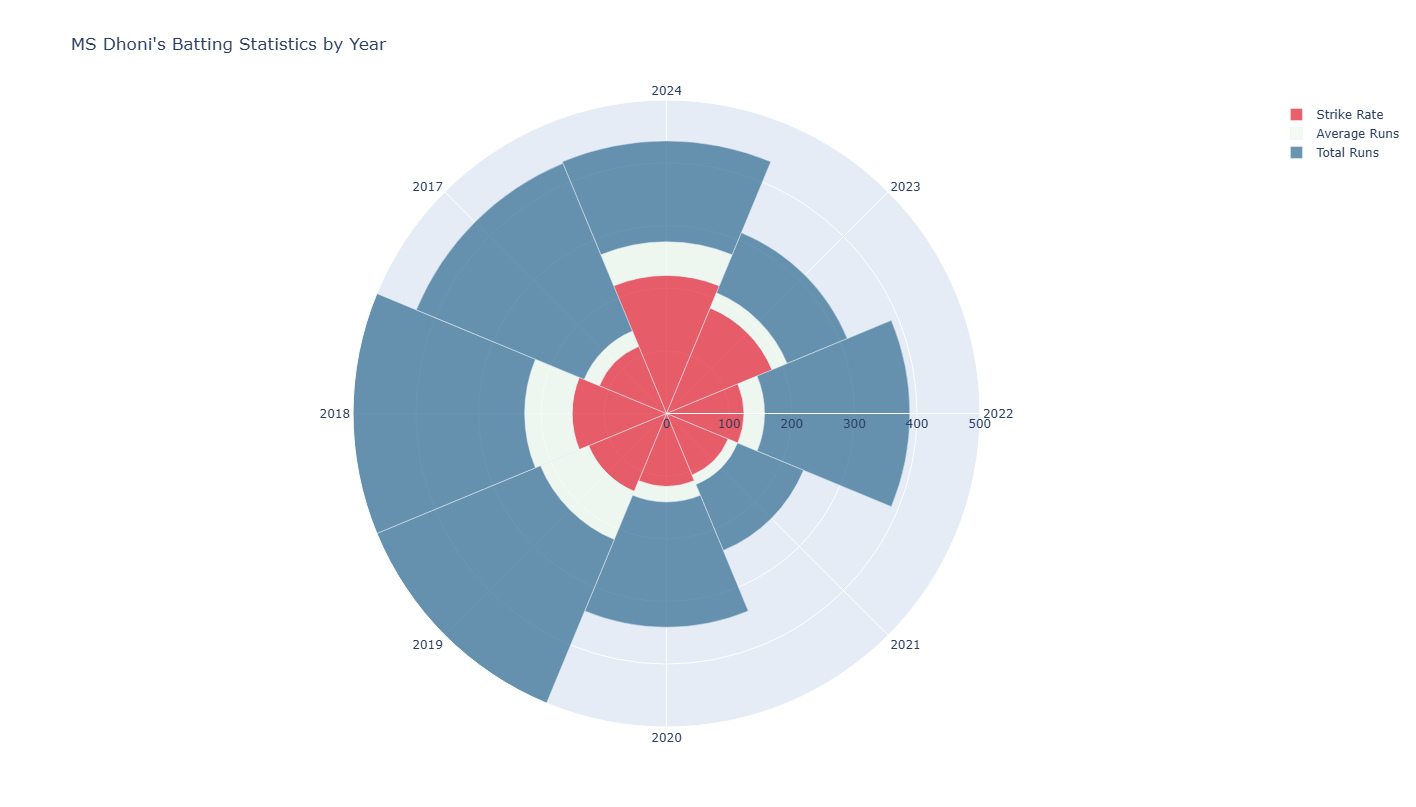
\includegraphics[width=0.85\linewidth]{img/coxcomb.png}
		      \caption{Coxcomb Plot, data from \cite{IPLT20CSKSquad}}
	      \end{figure}


\end{itemize}

\section{Monalisa}
First, the image is read using \texttt{matplotlib}'s \texttt{imread()} method.
Then we run a for loop for the shift amount and use \texttt{numpy}'s slicing to shift the image.
After, the shifted image is obtained, it's correlation with the original image is calculated using \texttt{numpy}'s \texttt{corrcoef()} method.
The shift amount is stored in \texttt{correlations\_x} and the correlation value is stored in \texttt{correlations\_y}.
Finally, a plot is made using \texttt{matplotlib}'s \texttt{plot()} method.

\begin{figure}[H]
	\centering
	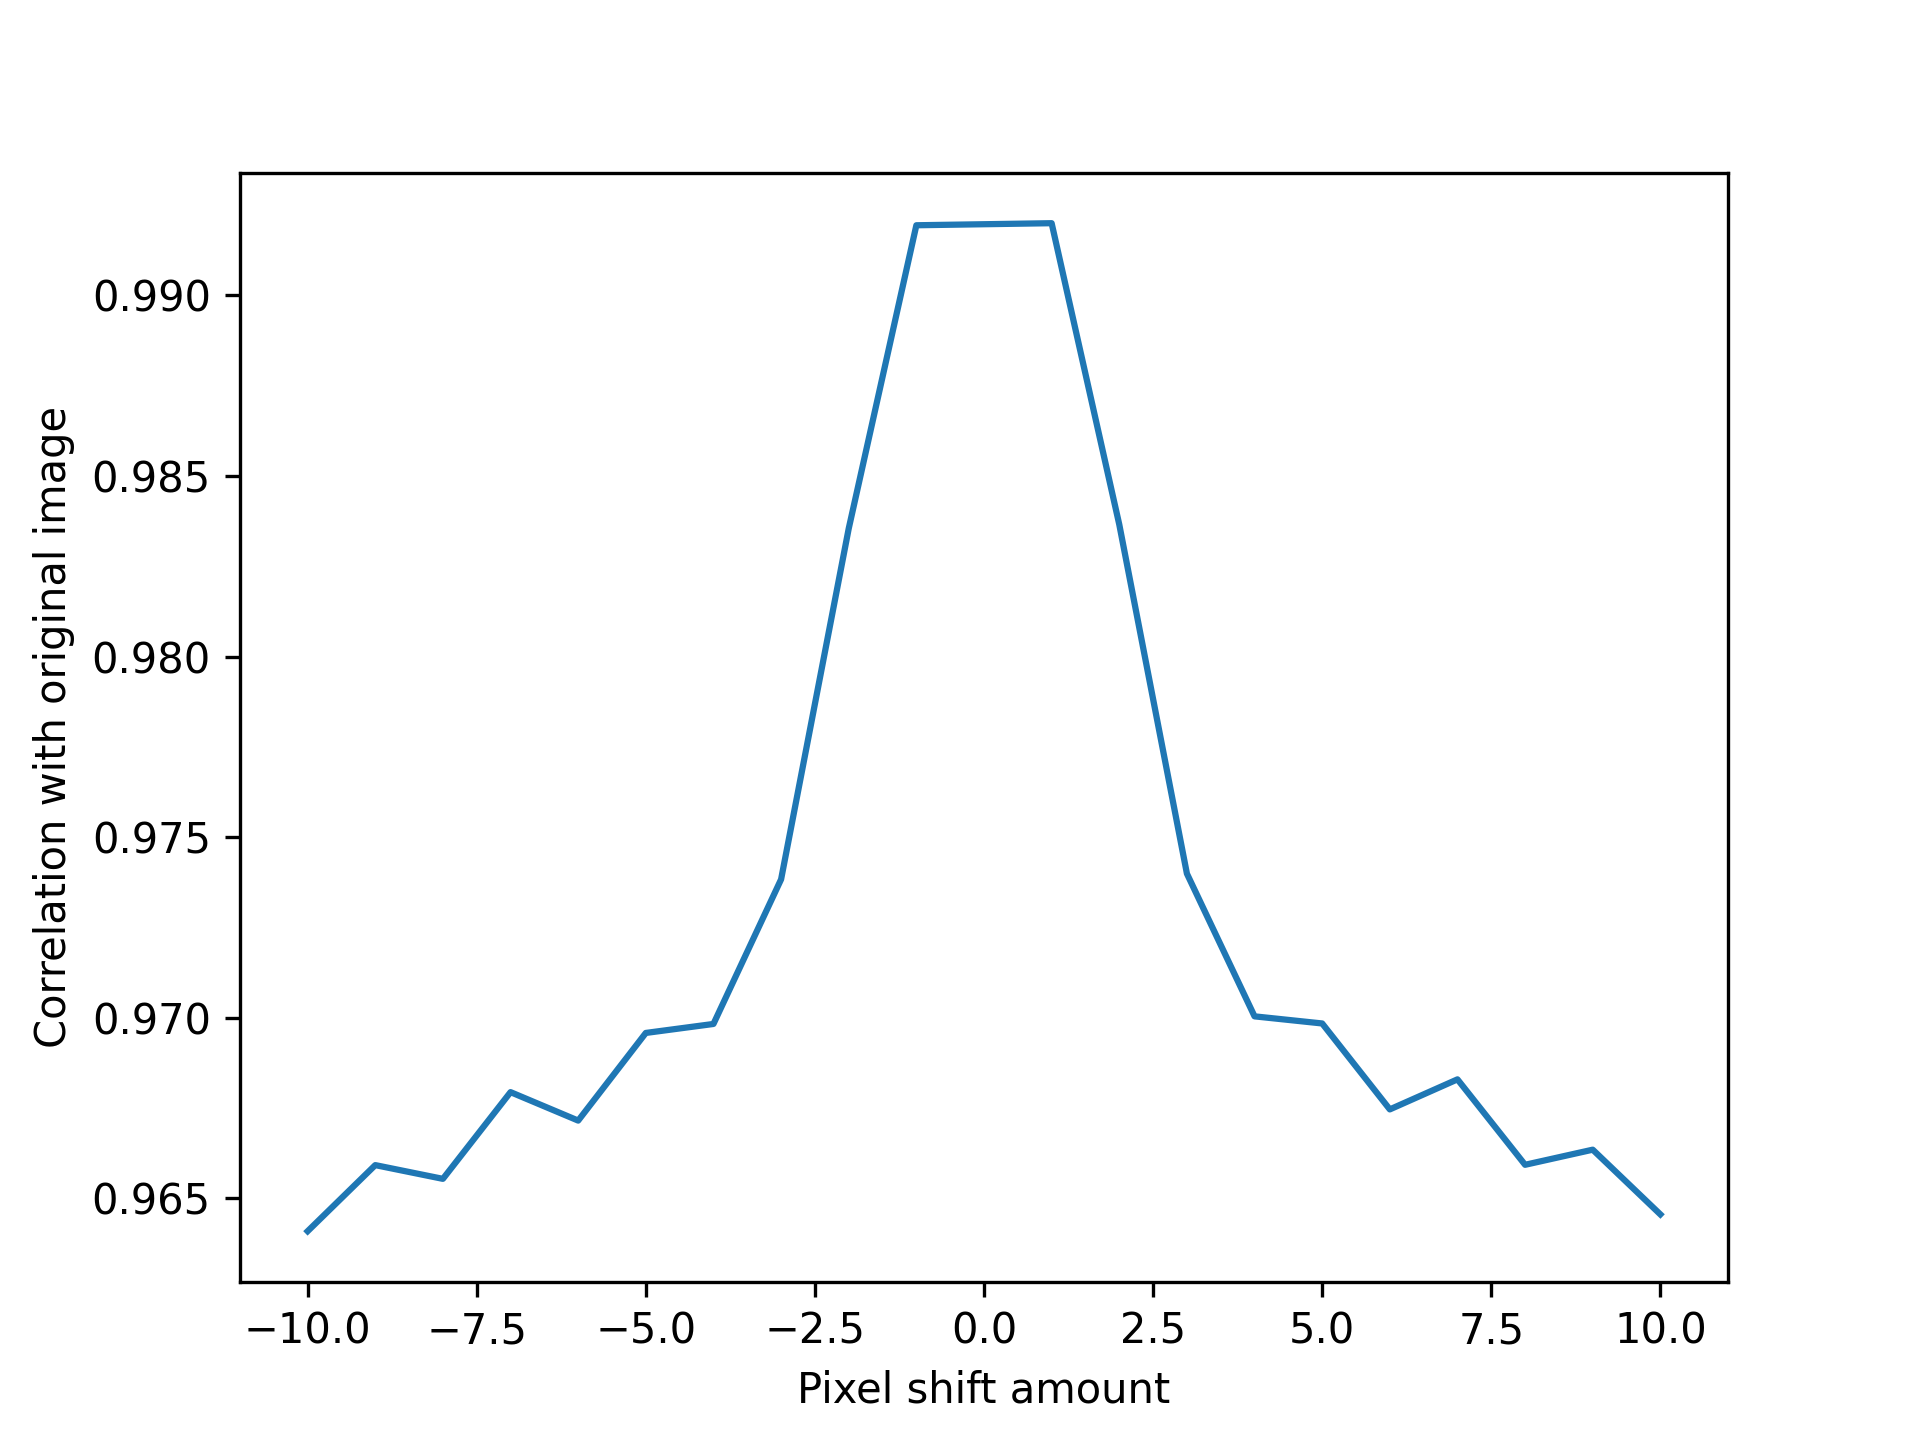
\includegraphics[width=0.8\textwidth]{img/correlation.png}
	\caption{Plot of correlation values against the pixel shift amounts}
	\label{fig:correlation}
\end{figure}

\begin{lstlisting}[language=Python, caption={Python code to compute and plot the correlations of the shifted images}, label=lst:correlation]
# imports
import numpy as np
import matplotlib.pyplot as plt

plt.rcParams["figure.dpi"] = 300  # higher resolution output images

img = plt.imread("Mona_Lisa.jpg")  # read the image

plt.imshow(img)
plt.gca().set_xlabel("x")  # set the x-label of the current Axes (returned by the gca)
plt.gca().set_ylabel("y")  # set the y-label of the current Axes

correlations_x = np.array(
    list(range(-10, 0)) + list(range(1, 11))
)  # x axis values for correlation plot
correlations_y = np.zeros(20)  # y axis values for correlation plot

for k in range(20):
    tx = correlations_x[k]  # shift amount
    img_new = np.zeros_like(img, dtype=np.uint8)  # create a new image
    if tx >= 0:
        img_new[:, tx:] = img[:, : img.shape[1] - tx]
    else:
        img_new[:, : img.shape[1] + tx] = img[:, -tx:]
    correlations_y[k] = np.corrcoef(img.flatten(), img_new.flatten())[
        0, 1
    ]  # store correlation

# plot the correlations
plt.figure()
plt.plot(correlations_x, correlations_y)
plt.xlabel("Pixel shift amount")
plt.ylabel("Correlation with original image")
plt.savefig("correlation.png")
\end{lstlisting}

The plot obtained is shown in \Cref{fig:correlation}.
We can see that the correlation between the original image and the shifted image decreases as the shift amount increases.
This is because adjacent pixels in the image have higher correlation as compared to pixels that are apart. In high resolution images, colors transition smoothly (without an abrupt change) between adjacent pixels.
This is easy to observe from \Cref{fig:shifted_images}.


\begin{figure}[H]
	\centering
	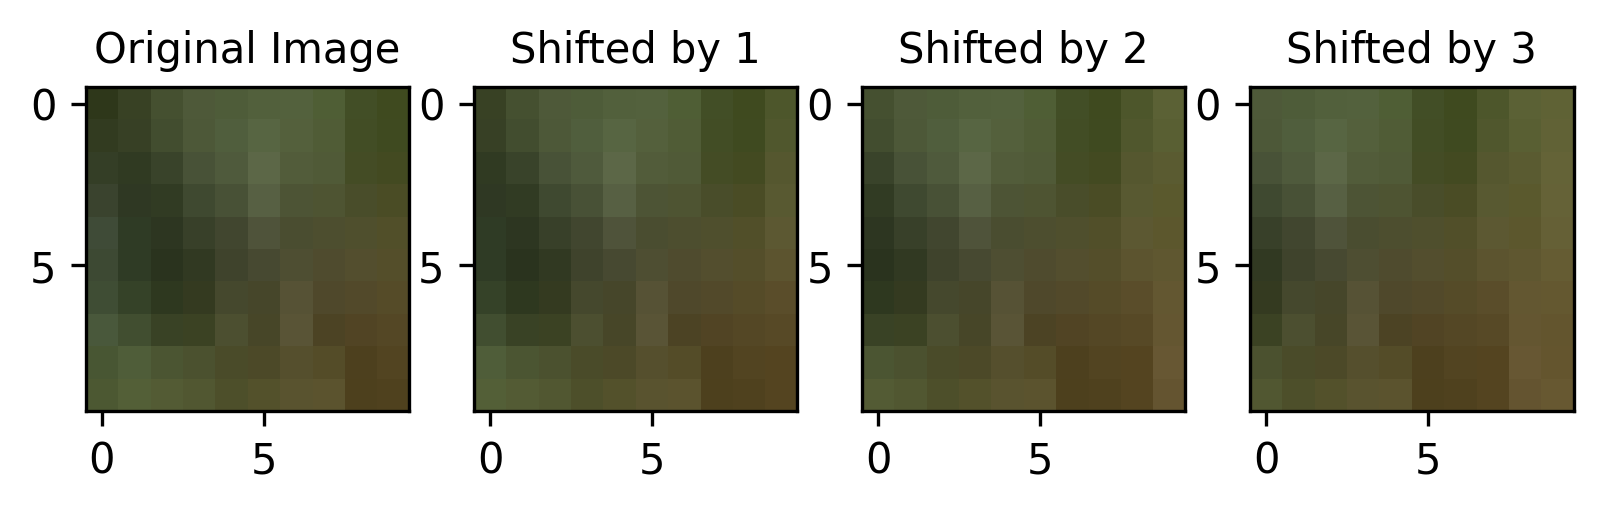
\includegraphics{img/shifted_images.png}
	\caption{Top left 10x10 pixels of the original and shifted images}
	\label{fig:shifted_images}
\end{figure}

To obtain the histogram of the image, we first convert the image to grayscale to get pixel intensities.
This is done using the formula
\[I = 0.2989 \times R + 0.5870 \times G + 0.1140 \times B\]
Then we use two for loops to iterate over all the pixels in the image, and calculate the histogram (frequency of each pixel intensity), which is stoed in variable \texttt{h}.
The histogram is then normalised by dividing by the total number of pixels in the image, this is soted in the variable \texttt{p}.
Finally, the histogram is plotted using \texttt{matplotlib}'s \texttt{hist()} method, but by using the \texttt{weights} parameter as we've already computed the histogram.
The output is shown in \Cref{fig:normalized_histogram}.

\begin{figure}[H]
	\centering
	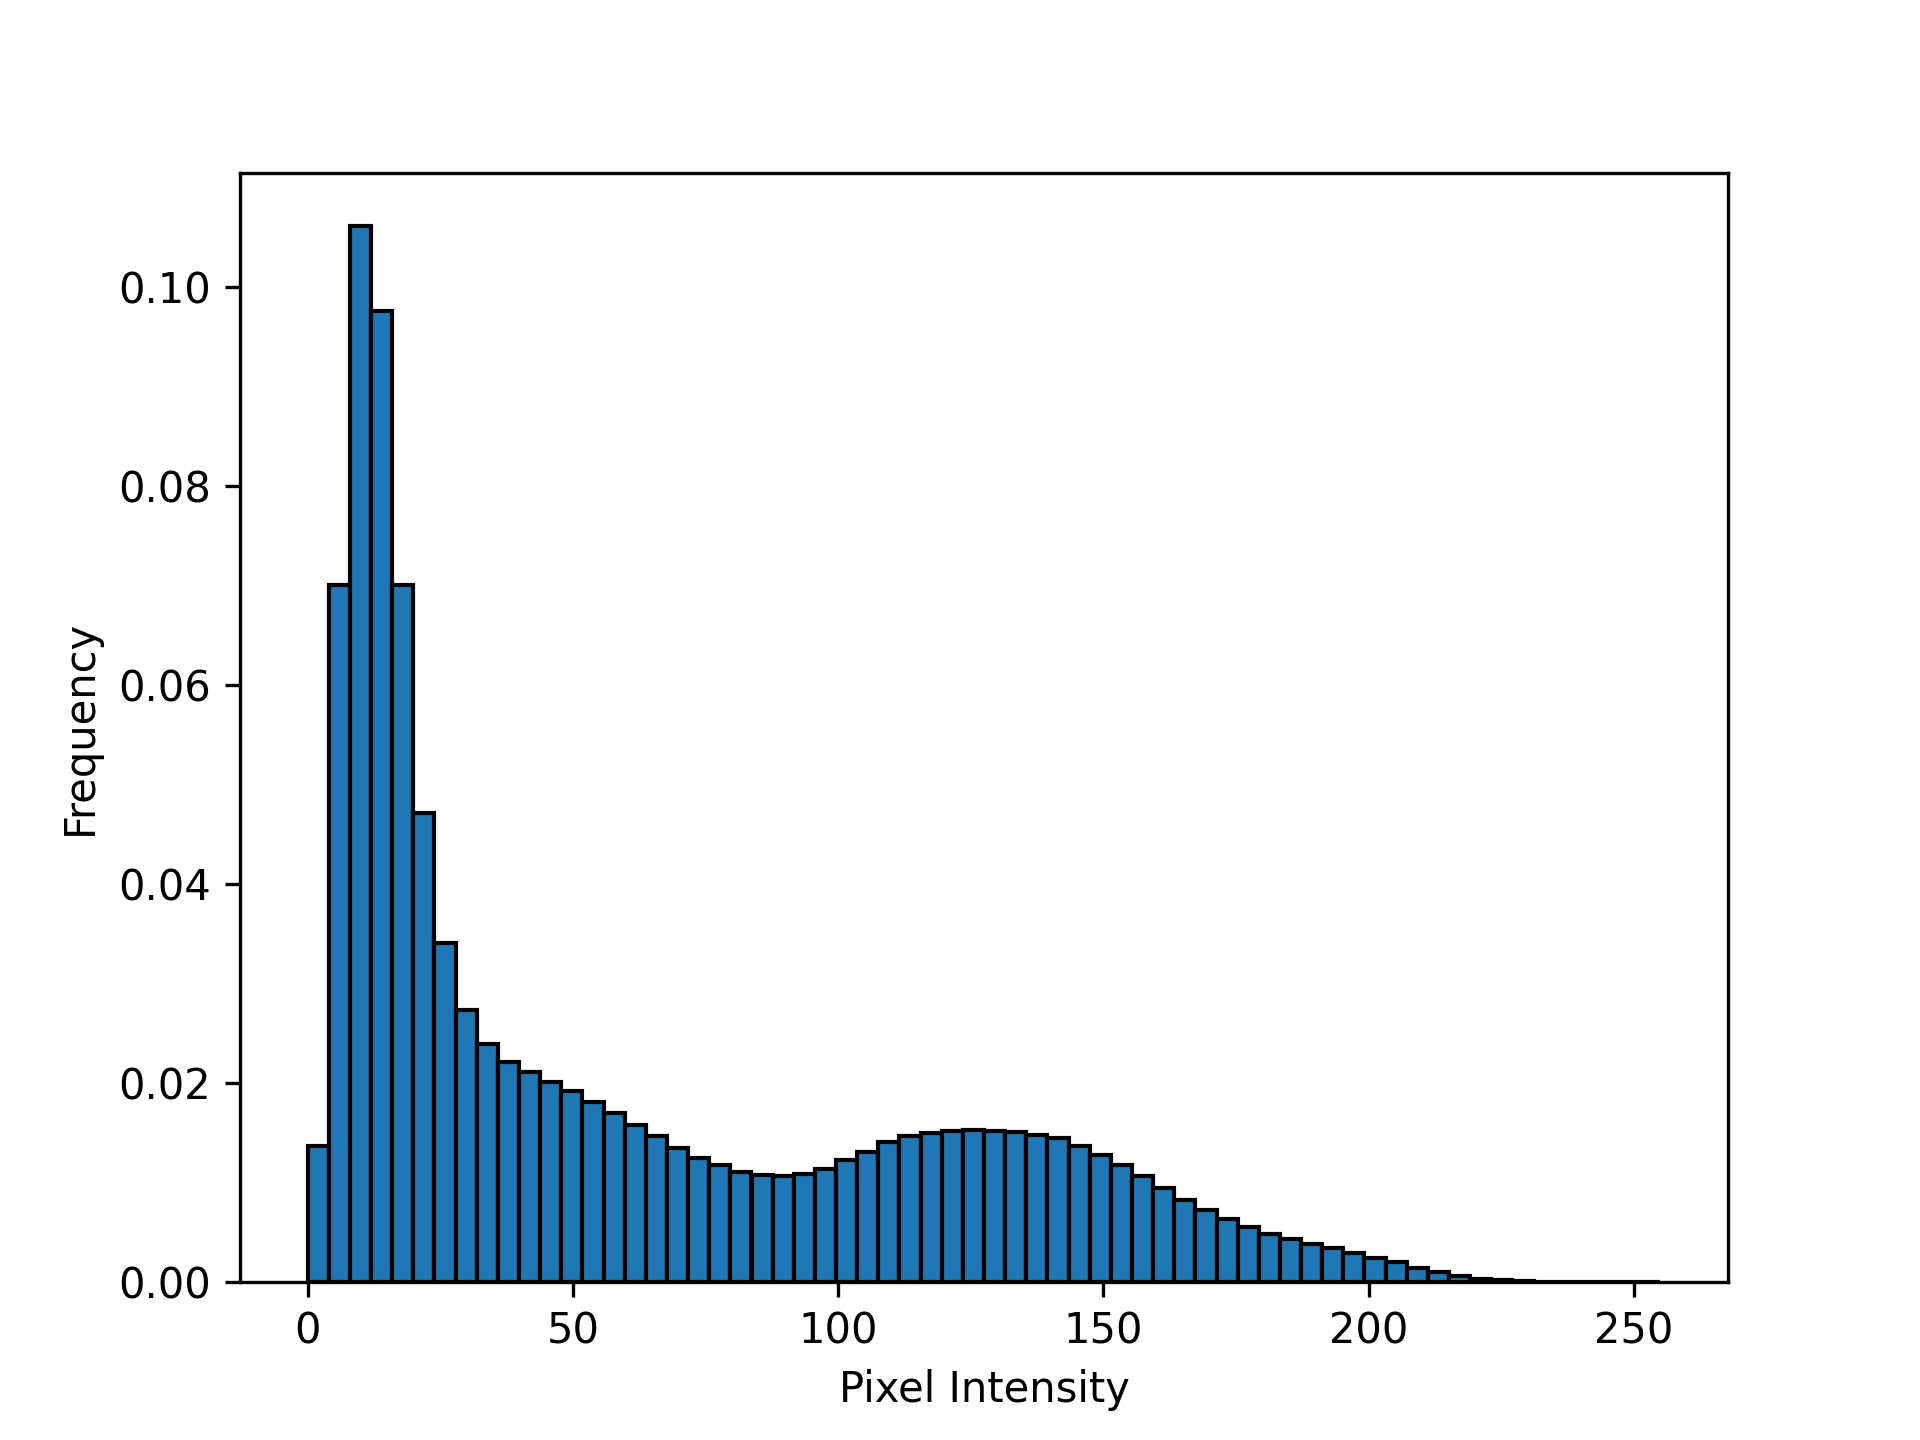
\includegraphics[width=0.8\textwidth]{img/normalized_histogram.png}
	\caption{Normalized histogram of the image}
	\label{fig:normalized_histogram}
\end{figure}

\begin{lstlisting}[language=Python, caption={Continuation of Listing \ref{lst:correlation}, to compute and plot the normalised histogram}]
# grayscale image for pixel intensities
img_gray = img[:, :, 0] * 0.2989 + img[:, :, 1] * 0.5870 + img[:, :, 2] * 0.1140
plt.imshow(img_gray, cmap="gray")

# histogram
h = np.zeros(256)
for i in range(img.shape[0]):
    for j in range(img.shape[1]):
        h[int(img_gray[i, j])] += 1
# normalized histogram
p = h / (img_gray.shape[0] * img_gray.shape[1])

# plot the normalized histogram
plt.figure()
_ = plt.hist(np.arange(256), weights=p, bins=64, edgecolor="black")
plt.xlabel("Pixel Intensity")
plt.ylabel("Frequency")
plt.savefig("normalized_histogram.png")
\end{lstlisting}


\footnotetext{Running Instructions: \texttt{python ./file\_name.py}}

\newpage
\nocite{*}
\addcontentsline{toc}{section}{Bibliography}

\bibliographystyle{plainurl}
\bibliography{references}
\end{document}
